% Options for packages loaded elsewhere
% Options for packages loaded elsewhere
\PassOptionsToPackage{unicode}{hyperref}
\PassOptionsToPackage{hyphens}{url}
\PassOptionsToPackage{dvipsnames,svgnames,x11names}{xcolor}
%
\documentclass[
  12pt,
  letterpaper,
  DIV=11,
  numbers=noendperiod]{scrartcl}
\usepackage{xcolor}
\usepackage[margin=1in]{geometry}
\usepackage{amsmath,amssymb}
\setcounter{secnumdepth}{-\maxdimen} % remove section numbering
\usepackage{iftex}
\ifPDFTeX
  \usepackage[T1]{fontenc}
  \usepackage[utf8]{inputenc}
  \usepackage{textcomp} % provide euro and other symbols
\else % if luatex or xetex
  \usepackage{unicode-math} % this also loads fontspec
  \defaultfontfeatures{Scale=MatchLowercase}
  \defaultfontfeatures[\rmfamily]{Ligatures=TeX,Scale=1}
\fi
\usepackage{lmodern}
\ifPDFTeX\else
  % xetex/luatex font selection
\fi
% Use upquote if available, for straight quotes in verbatim environments
\IfFileExists{upquote.sty}{\usepackage{upquote}}{}
\IfFileExists{microtype.sty}{% use microtype if available
  \usepackage[]{microtype}
  \UseMicrotypeSet[protrusion]{basicmath} % disable protrusion for tt fonts
}{}
\usepackage{setspace}
\makeatletter
\@ifundefined{KOMAClassName}{% if non-KOMA class
  \IfFileExists{parskip.sty}{%
    \usepackage{parskip}
  }{% else
    \setlength{\parindent}{0pt}
    \setlength{\parskip}{6pt plus 2pt minus 1pt}}
}{% if KOMA class
  \KOMAoptions{parskip=half}}
\makeatother
% Make \paragraph and \subparagraph free-standing
\makeatletter
\ifx\paragraph\undefined\else
  \let\oldparagraph\paragraph
  \renewcommand{\paragraph}{
    \@ifstar
      \xxxParagraphStar
      \xxxParagraphNoStar
  }
  \newcommand{\xxxParagraphStar}[1]{\oldparagraph*{#1}\mbox{}}
  \newcommand{\xxxParagraphNoStar}[1]{\oldparagraph{#1}\mbox{}}
\fi
\ifx\subparagraph\undefined\else
  \let\oldsubparagraph\subparagraph
  \renewcommand{\subparagraph}{
    \@ifstar
      \xxxSubParagraphStar
      \xxxSubParagraphNoStar
  }
  \newcommand{\xxxSubParagraphStar}[1]{\oldsubparagraph*{#1}\mbox{}}
  \newcommand{\xxxSubParagraphNoStar}[1]{\oldsubparagraph{#1}\mbox{}}
\fi
\makeatother


\usepackage{longtable,booktabs,array}
\usepackage{calc} % for calculating minipage widths
% Correct order of tables after \paragraph or \subparagraph
\usepackage{etoolbox}
\makeatletter
\patchcmd\longtable{\par}{\if@noskipsec\mbox{}\fi\par}{}{}
\makeatother
% Allow footnotes in longtable head/foot
\IfFileExists{footnotehyper.sty}{\usepackage{footnotehyper}}{\usepackage{footnote}}
\makesavenoteenv{longtable}
\usepackage{graphicx}
\makeatletter
\newsavebox\pandoc@box
\newcommand*\pandocbounded[1]{% scales image to fit in text height/width
  \sbox\pandoc@box{#1}%
  \Gscale@div\@tempa{\textheight}{\dimexpr\ht\pandoc@box+\dp\pandoc@box\relax}%
  \Gscale@div\@tempb{\linewidth}{\wd\pandoc@box}%
  \ifdim\@tempb\p@<\@tempa\p@\let\@tempa\@tempb\fi% select the smaller of both
  \ifdim\@tempa\p@<\p@\scalebox{\@tempa}{\usebox\pandoc@box}%
  \else\usebox{\pandoc@box}%
  \fi%
}
% Set default figure placement to htbp
\def\fps@figure{htbp}
\makeatother





\setlength{\emergencystretch}{3em} % prevent overfull lines

\providecommand{\tightlist}{%
  \setlength{\itemsep}{0pt}\setlength{\parskip}{0pt}}



 
\usepackage[backend=biber,style=apa,sorting=nyt,maxcitenames=2]{biblatex}
\addbibresource{../references/references.bib}
\addbibresource{../references/MyLibrary2025-08-25.bib}


\usepackage{amsthm,amsmath,amsfonts,amssymb,float,caption,subcaption}
\usepackage{pdflscape}
\DeclareLanguageMapping{english}{english-apa}
\KOMAoption{captions}{tableheading}
\makeatletter
\@ifpackageloaded{caption}{}{\usepackage{caption}}
\AtBeginDocument{%
\ifdefined\contentsname
  \renewcommand*\contentsname{Table of contents}
\else
  \newcommand\contentsname{Table of contents}
\fi
\ifdefined\listfigurename
  \renewcommand*\listfigurename{List of Figures}
\else
  \newcommand\listfigurename{List of Figures}
\fi
\ifdefined\listtablename
  \renewcommand*\listtablename{List of Tables}
\else
  \newcommand\listtablename{List of Tables}
\fi
\ifdefined\figurename
  \renewcommand*\figurename{Figure}
\else
  \newcommand\figurename{Figure}
\fi
\ifdefined\tablename
  \renewcommand*\tablename{Table}
\else
  \newcommand\tablename{Table}
\fi
}
\@ifpackageloaded{float}{}{\usepackage{float}}
\floatstyle{ruled}
\@ifundefined{c@chapter}{\newfloat{codelisting}{h}{lop}}{\newfloat{codelisting}{h}{lop}[chapter]}
\floatname{codelisting}{Listing}
\newcommand*\listoflistings{\listof{codelisting}{List of Listings}}
\makeatother
\makeatletter
\makeatother
\makeatletter
\@ifpackageloaded{caption}{}{\usepackage{caption}}
\@ifpackageloaded{subcaption}{}{\usepackage{subcaption}}
\makeatother
\usepackage{bookmark}
\IfFileExists{xurl.sty}{\usepackage{xurl}}{} % add URL line breaks if available
\urlstyle{same}
\hypersetup{
  pdftitle={Quantifying Hidden Exploitation: Dual-Method Prevalence Estimates of Labour Exploitation among Domestic Workers in the United Kingdom},
  pdfauthor={Caroline Emberson; Scott Moser},
  pdfkeywords={social indicators, SDG 8.7, labour exploitation, migrant
domestic work, respondent-driven sampling, network scale-up method},
  colorlinks=true,
  linkcolor={black},
  filecolor={Maroon},
  citecolor={RoyalBlue},
  urlcolor={BrickRed},
  pdfcreator={LaTeX via pandoc}}


\title{Quantifying Hidden Exploitation: Dual-Method Prevalence Estimates
of Labour Exploitation among Domestic Workers in the United Kingdom}
\author{Caroline Emberson \and Scott Moser}
\date{25 June 2026}
\begin{document}
\maketitle
\begin{abstract}
Reliable indicators for SDG Target 8.7 are difficult to construct
because the populations most affected by labour exploitation are often
absent from standard household and labour-force surveys. This paper
develops a matched ego/alter survey design for measuring labour
exploitation among hidden populations. We apply respondent-driven
sampling and a network scale-up approach to the same survey instrument,
asking migrant domestic workers in the United Kingdom both about their
own experiences and about exploitation among domestic workers they know.
The design produces two complementary estimands: own-experience
prevalence and network-visible prevalence. We measure five ILO-aligned
indicators: excessive working hours, pay-related issues, limited access
to help, threats and abuse, and document withholding. We also construct
a formative composite risk index to capture gradations of exploitation
severity. In a civil-society-mediated web-RDS sample of 85 migrant
domestic workers, RDS-SS estimates indicate high own-experience
prevalence, while network scale-up estimates are substantially lower.
The divergence is consistent with a visibility gradient in which some
exploitation behaviours are more observable across peer networks than
others. The results should be interpreted as exploratory
population-adjusted estimates for an RDS-reachable population rather
than definitive national prevalence figures. The paper contributes a
replicable measurement design for hidden-population social indicators
relevant to SDG 8.7 monitoring.
\end{abstract}


\setstretch{1.15}
\section{Introduction}\label{introduction}

Modern slavery --- forced labour, debt bondage, document and
identity-document withholding, and related coercive practices --- is
named under Sustainable Development Goal Target 8.7 as a priority for
elimination by 2030. Reliable prevalence measurement is a precondition
for monitoring that target, yet the populations most affected are
largely invisible to the household and labour-force surveys on which
official social indicators rely. Conventional household surveys
underestimate prevalence in this domain by an order of magnitude or
more, both because the populations affected (undocumented migrants,
live-in domestic workers, sex workers, agricultural day labourers) are
excluded from sampling frames, and because exploitation behaviours ---
especially those at the more severe end of the spectrum --- are
typically not self-reported even when the respondent is contacted. The
civil-society and grey-literature evidence base on UK domestic workers
(Kalayaan 2008; Latin American Women's Rights Service 2023) is
qualitatively rich but does not yield population-level prevalence
estimates suitable for SDG monitoring or comparison across populations.
The International Labour Organization's eleven indicators of forced
labour (ILO 2012, 2017) provide an operational framework for measuring
modern slavery, but the empirical question of which indicators are
observable through which survey design remains open. Studies typically
apply one design --- household survey, respondent-driven sampling (RDS),
or the network scale-up method (NSUM) --- and report prevalence
accordingly. None to our knowledge applies both RDS and NSUM to the same
survey instrument for the same indicators, the design that would allow
direct triangulation of ego-based against alter-based estimates and,
where the two diverge, diagnostic inference about which exploitation
behaviours are visible within personal networks and which are not.

This paper makes two contributions. First, we apply RDS and NSUM to the
same survey instrument with the same respondents, eliciting ego-based
and alter-based estimates of an identical set of five ILO-aligned
indicators. The dual-method design produces two complementary estimands
(own-experience prevalence from RDS, network-visible prevalence from
NSUM); where they diverge, the gap is itself diagnostic evidence about
the visibility gradient of different exploitation behaviours within
workers' personal networks. Second, we operationalise modern slavery as
a graded hierarchy of indicators rather than a binary condition,
organised around the ILO's operational distinction (ILO 2012, 2017)
between `medium' indicators (multiple required to indicate forced
labour) and `strong' indicators (any one alone sufficient). This
hierarchy lets a single survey instrument capture exploitation across
the full spectrum of severity and supports a continuous formative
additive composite risk index. Taken together, the contribution of the
paper is best read as developing and demonstrating a defensible
social-indicator measurement strategy for hidden-population exploitation
rather than as producing a definitive national prevalence estimate. We
demonstrate the strategy with a respondent-driven sample of 85 UK
migrant domestic workers and discuss how the methodology generalises to
other hidden populations relevant to SDG 8.7 monitoring.

The remainder of the paper is organised as follows. Section 2
conceptualises labour exploitation as a graded latent construct measured
by five ILO-aligned indicators arranged hierarchically by severity.
Section 3 describes the matched-instrument survey design (Section 3.1)
and the dual sampling approach combining RDS and NSUM (Section 3.2).
Section 4 presents prevalence estimates by indicator and method,
including frequentist RDS-I/RDS-II/RDS-SS estimators (Section 4.1),
Bayesian Model-Assisted inference (Section 4.2), and NSUM with
continuous-\(\tau\) sensitivity analysis (Section 4.3). Section 5 reads
the RDS-NSUM divergence as diagnostic evidence about visibility within
workers' personal networks and discusses implications for SDG 8.7
monitoring.

\section{Conceptualising Labour Exploitation and the Degree of
Risk}\label{conceptualising-labour-exploitation-and-the-degree-of-risk}

The International Labour Organization's eleven indicators of forced
labour (ILO 2012, 2017) provide the canonical operational framework for
measuring modern slavery. The ILO distinguishes two grades of indicator:
`medium' indicators (excessive overtime, wage withholding, debt bondage,
restriction of movement, isolation, abusive working and living
conditions, abuse of vulnerability, deception) whose presence
individually is suggestive but not definitive of forced labour, and
`strong' indicators (intimidation and threats, physical and sexual
violence, retention of identity documents) any one of which alone is
sufficient to indicate forced labour. This medium/strong distinction is
itself a graded hierarchy of evidentiary weight, not a binary. We
measure five indicators across that hierarchy, chosen to span the ILO
conceptual space efficiently within the constraints of a
matched-instrument ego/alter survey design. Three are medium indicators
--- excessive working hours, pay-related issues (combining wage
withholding with elements of debt bondage), and limited access to help
(combining restriction of movement with isolation, as both manifest in
the same observable behaviour in the domestic-work context). Two are
strong indicators --- threats and abuse (combining intimidation/threats
with physical and sexual violence, which prior qualitative work suggests
co-occur in this population: Yilmaz and Emberson 2023) and document and
passport withholding. The remaining two ILO indicators --- abuse of
vulnerability and deception --- are not measured as standalone binary
prevalence indicators: both are too retrospective and judgemental to
elicit reliably through a brief survey of n=85 respondents (the
respondent would need to reconstruct intent and knowledge states from
the perspective of months or years after the fact). Both are nonetheless
included in the composite risk index (Section 4.2; ESM\_1 Table 1,
Categories 1 and 2). Where appropriate we note this scope limitation in
the discussion of results.

The composite risk index we construct is a formative additive composite
in the sense of Diamantopoulos and Siguaw (2006) and Mazziotta and
Pareto (2013, 2016), aggregating all eleven ILO indicators of forced
labour into a single continuous quality-of-life-relevant measure (see
Section 3.2, Table 1 for the indicator-to-category mapping; ESM\_1 Table
1 for per-category weights). The composite is formative rather than
reflective: an individual is exploited if they are subject to any of
these conditions, and the conditions are constitutive rather than
reflective of an underlying latent severity (Diamantopoulos and Siguaw
2006; Diamantopoulos et al.~2008). Polarity is uniform across categories
--- each indicator has the same direction with respect to the latent
construct of exploitation severity. The choice of aggregation follows
the guidance of Maggino (2017) and the SIR editorial team (Bartram et
al.~2024): we use a weighted additive index in which weights are
anchored on the ILO medium/strong severity gradation (strong-indicator
categories receive larger sub-weights than medium-indicator categories),
and we conduct robustness assessment by perturbing the weights (Section
5.5). Two further evidentiary markers --- NRM-referral history and
payment below the national living wage --- are reported as separate
binary flags and are not part of the composite, as their direct
evidentiary status under UK policy makes them more useful read
independently of the composite construction.

\subsection{2.1 Evaluating the Degree of
Risk}\label{evaluating-the-degree-of-risk}

We conceptualise risk of labour exploitation from the workers'
perspective, spanning a spectrum from illegal employment practices
(below-minimum-wage payment, health and safety violations) through to
forced labour and modern slavery. The more ILO indicators present, the
stronger the likelihood of exploitation. We operationalise this in two
complementary ways: binary indicators classifying respondents as
exploited or not on each ILO-aligned dimension (threshold criteria,
Section 4.3) and a continuous formative additive composite risk index
capturing gradations of vulnerability across all eleven ILO indicators
(Section 4.2; ESM\_1 for full construction).

\section{Case Setting: Labour Exploitation Risk Among Transnational
Migrant Domestic Workers In The
UK}\label{case-setting-labour-exploitation-risk-among-transnational-migrant-domestic-workers-in-the-uk}

Domestic work in the United Kingdom is performed predominantly by
transnational migrant women, the majority entering on tied Overseas
Domestic Worker (ODW) visas under which the right to remain is
conditional on employment with a specific employer (Mantouvalou 2016;
Kalayaan 2008; Latin American Women's Rights Service 2023). The
combination of tied immigration status, work performed inside the
private home, and the absence of routine workplace inspection creates
structural conditions under which labour exploitation can occur
unobserved by employment regulators, mainstream labour-market surveys,
and the police (Romero and Fisher 2025). Civil-society organisations
representing migrant domestic workers have documented patterns of wage
withholding, document confiscation, restricted movement, excessive
working hours, and threats and abuse over more than two decades
(Kalayaan 2008; Mantouvalou 2016; Latin American Women's Rights Service
2023; Yilmaz and Emberson 2023), but the qualitative and case-based
evidence base has not yielded population-level prevalence estimates
suitable for SDG 8.7 monitoring or cross-population comparison. The UK
migrant domestic worker case is therefore well-suited as the testbed for
a measurement methodology aimed at producing comparable prevalence
indicators for hidden, civil-society-mediated populations relevant to
SDG 8.7 reporting. The methodology demonstrated here generalises to
other hidden populations sharing the structural features of tied
employment, private-home workplaces, and civil-society-mediated access
(undocumented agricultural workers, kafala-system migrants in Gulf
states, informal-construction day labourers).

\subsection{3.1 Study Design and
Sampling}\label{study-design-and-sampling}

Respondent-Driven Sampling (RDS) is a network-based sampling method
designed to study hidden or hard-to-reach populations (Heckathorn, 1997,
2011; Gile \emph{et al.}, 2018). It combines chain-referral sampling
with a statistical framework to produce population estimates that adjust
for network structure and differential recruitment probabilities. The
method begins with a set of initial participants (``seeds''), who
recruit peers from their social networks. Recruits, in turn, recruit
others, creating waves of participation. Each participant reports their
network degree (the number of eligible contacts they know), which is
used to adjust for selection bias---especially the oversampling of
high-degree individuals.

RDS has been widely used to sample hidden populations in public health
and social science research (McCreesh \emph{et al.}, 2012; Schwitters,
Swaminathan and Serwadda, 2012), and network-based referrals have been
described as the only viable method to reach many types of labour
trafficking victims (Zhang, 2012). Recent applications include studies
of exploitation among low-wage workers in American cities (Bernhardt,
Milkman, and N., 2009), labour trafficking in migrant communities
(Vincent and Thompson, 2017), child labour in India (Zhang \emph{et
al.}, 2019), and commercial sexual exploitation in Nepal (Jordan
\emph{et al.}, 2020).

Our approach can best be described as Web-based RDS (Wejnert and
Heckathorn, 2008). We designed a web survey using the JISC online survey
interface, suitable for respondents to complete via mobile phone. The
main survey was conducted over five months between February and July
2023.

\emph{Seed Selection and Recruitment}

We selected our first wave of participants nonrandomly by convenience
sampling. Mobile phone numbers were used both to identify seed
participants and to act as a unique identifier for those whom they
referred. To avoid sample homophily, original sample members were
selected from three distinct domestic worker communities facilitated by
civil society organisations. One was an exclusively online community of
transnational domestic workers working in the UK, the second represented
UK domestic workers of Filipino origin, and the third drew its
membership from the Latin American community of domestic workers, also
in the UK. Representatives from these organisations, along with other
academics with expertise in exploitation within domestic work,
contributed to survey question design and facilitated piloting of an
initial version of the survey, which was translated and made available
in four languages: English, Spanish, Tagalog, and Portuguese.

\emph{Incentive Design and Participation Verification}

A double incentive scheme rewarded respondents both for completing the
questionnaire and for each referral who went on to engage with the
survey. The challenge of incentive design is to set the incentive at a
level that adequately rewards respondents' time and participation, but
that also avoids the risk of fraudulent participation due to too high a
monetary gain (Jordan \emph{et al.}, 2020). A sum of £10 was provided
for survey completion with a further £5 for each successful nomination.
While respondents were asked to nominate up to 10 domestic workers
within their existing social network, participation from up to five of
these was requested in subsequent waves. This approach is akin to the
use of vouchers in face-to-face studies as advocated by Thompson (2020).

Respondents were incentivised through lottery entry, consistent with the
design recommendations of the survey-incentive literature (full
literature review and incentive-design details in ESM\_4 Section C).

\subsection{3.2 Survey Instrument and
Indicators}\label{survey-instrument-and-indicators}

The survey instrument was designed to capture both egocentric
(ego-based) and altercentric (alter-based) network information, enabling
the application of both RDS and NSUM estimation methods. Composite
measures to quantify the extent to which respondents were at risk of
labour exploitation, including severe forms of exploitation such as
forced labour, were constructed from existing exploitation typologies,
notably the ILO's Indicators of Forced Labour (I.L.O., 2012). The eleven
ILO indicators of forced labour (ILO 2012, 2017) provide the operational
framework for our measurement strategy. Table 1 (below) maps each ILO
indicator to its measurement status in this paper: whether it is
measured directly as a binary prevalence indicator (reported in Section
4.3), whether it is included in the formative additive composite risk
index (reported in Section 4.2), and which survey questions elicit the
ego- and alter-based reports.

\begin{longtable}[]{@{}
  >{\raggedleft\arraybackslash}p{(\linewidth - 10\tabcolsep) * \real{0.0364}}
  >{\raggedright\arraybackslash}p{(\linewidth - 10\tabcolsep) * \real{0.3545}}
  >{\centering\arraybackslash}p{(\linewidth - 10\tabcolsep) * \real{0.0909}}
  >{\raggedright\arraybackslash}p{(\linewidth - 10\tabcolsep) * \real{0.2364}}
  >{\centering\arraybackslash}p{(\linewidth - 10\tabcolsep) * \real{0.1000}}
  >{\raggedright\arraybackslash}p{(\linewidth - 10\tabcolsep) * \real{0.1818}}@{}}
\caption{Mapping of the eleven ILO Indicators of Forced Labour to this
paper's measurement scheme. The five binary prevalence indicators
(right-hand grouping in column 4: document withholding, threats and
abuse, pay-related issues, limited access to help, excessive working
hours) jointly cover nine of the eleven ILO indicators (all except abuse
of vulnerability and deception, which are captured in the composite
only). The composite risk index covers all eleven ILO indicators through
eleven weighted sub-categories. Two further evidentiary markers ---
NRM-referral history (Q80) and payment below the national living wage
(Q36) --- are reported as separate binary flags and are not part of the
composite. Full per-category weight values are given in ESM\_1, Table 1.
Source: Authors' construction following ILO (2012,
2017).}\tabularnewline
\toprule\noalign{}
\begin{minipage}[b]{\linewidth}\raggedleft
\#
\end{minipage} & \begin{minipage}[b]{\linewidth}\raggedright
ILO indicator (2012, 2017)
\end{minipage} & \begin{minipage}[b]{\linewidth}\centering
Severity
\end{minipage} & \begin{minipage}[b]{\linewidth}\raggedright
Binary indicator
\end{minipage} & \begin{minipage}[b]{\linewidth}\centering
Composite
\end{minipage} & \begin{minipage}[b]{\linewidth}\raggedright
Survey item(s)
\end{minipage} \\
\midrule\noalign{}
\endfirsthead
\toprule\noalign{}
\begin{minipage}[b]{\linewidth}\raggedleft
\#
\end{minipage} & \begin{minipage}[b]{\linewidth}\raggedright
ILO indicator (2012, 2017)
\end{minipage} & \begin{minipage}[b]{\linewidth}\centering
Severity
\end{minipage} & \begin{minipage}[b]{\linewidth}\raggedright
Binary indicator
\end{minipage} & \begin{minipage}[b]{\linewidth}\centering
Composite
\end{minipage} & \begin{minipage}[b]{\linewidth}\raggedright
Survey item(s)
\end{minipage} \\
\midrule\noalign{}
\endhead
\bottomrule\noalign{}
\endlastfoot
1 & Abuse of vulnerability & Medium & --- (composite only) & Cat 1 &
Q29, Q51 \\
2 & Deception & Medium & --- (composite only) & Cat 2 & Q45 \\
3 & Restriction of movement & Medium & Limited access to help & Cat 3 &
Q32, Q46 \\
4 & Isolation & Medium & Limited access to help & Cat 4 & Q65 \\
5 & Physical and sexual violence & Strong & Threats and abuse & Cat 5 &
Q44 (5c1, 5c1-b) \\
6 & Intimidation and threats & Strong & Threats and abuse & Cat 6 &
Q47 \\
7 & Retention of identity documents & Strong & Document withholding &
Cat 7 & Q70 \\
8 & Withholding of wages & Medium & Pay-related issues & Cat 8 & Q42 \\
9 & Debt bondage & Medium & Pay-related issues & Cat 9 & Q39 \\
10 & Abusive working and living conditions & Medium & Partial (Q48) &
Cat 10 & Q48, Q63, Q72, Q76 \\
11 & Excessive overtime & Medium & Excessive working hours & Cat 11 &
Q16, Q61, Q62 \\
\end{longtable}

Based on this mapping, we operationalise exploitation in two ways: (1)
five binary prevalence indicators classifying respondents as exploited
or not exploited on each dimension based on threshold criteria (Section
4.3), and (2) one continuous formative additive composite risk index
designed to capture gradations of vulnerability across the full sample
(Section 4.2).

Ego-based questions capture respondents' own experiences of exploitation
(used for RDS estimation), while alter-based questions ask respondents
to report on the exploitation experiences of domestic workers they know
(used for NSUM estimation). See Online Resource ESM\_1 and ESM\_2 for
details of these survey questions and the construction of comparable
ego- and alter-based indicators.

\subsection{3.3 Sample Characteristics}\label{sample-characteristics}

In total, we received completed online surveys from 97 respondents.
Twelve participants reported knowing zero domestic workers in the
UK---that is, having a null social network---and were excluded from RDS
analysis because network degree information is required for RDS
weighting procedures. This resulted in an analytical sample of 85
respondents for RDS-based estimation. Although the analytic sample
comprises 85 respondents, this is within the range used in comparable
respondent-driven sampling (RDS) and network scale-up (NSUM) studies of
hidden populations (Gile and Handcock, 2010; Goel and Salganik, 2010;
Gile, 2011). Statistical inference in these designs depends not on the
absolute sample size but on the structure of the recruitment network,
degree distribution, and convergence to equilibrium (Salganik and
Heckathorn, 2004). Furthermore, model-assisted and Bayesian RDS
estimators (Gile, 2011; Gile \emph{et al.}, 2018) provide valid
population estimates even for modest sample sizes, particularly when
uncertainty is appropriately quantified through resampling or posterior
distributions. In this study, we additionally employ a neighbourhood
bootstrap procedure that propagates sampling and network uncertainty,
providing robust confidence intervals consistent with small-sample
design-based inference (Handcock, Gile and Mar, 2014).

Of the 97 initial respondents, 90 identified themselves as transnational
migrants. Forty-five percent regarded themselves as self-employed, 39\%
identified themselves as employees, and 16\% categorised their
employment status as that of a worker. The largest single nationality
group, comprising 64 respondents (66\% of the total), reported a
Filipina background. Other nationalities represented included Dominican,
Brazilian, Spanish, Colombian, Bolivian, Venezuelan, Cuban, and
Panamanian. Female domestic workers made up 97\% of the sample, with 3\%
of the sample comprised of male domestic workers. The age structure of
the domestic workers was skewed towards those over 45 years old, with
such workers representing over half of the sample (see Table 1).

\begin{figure}[H]

{\centering 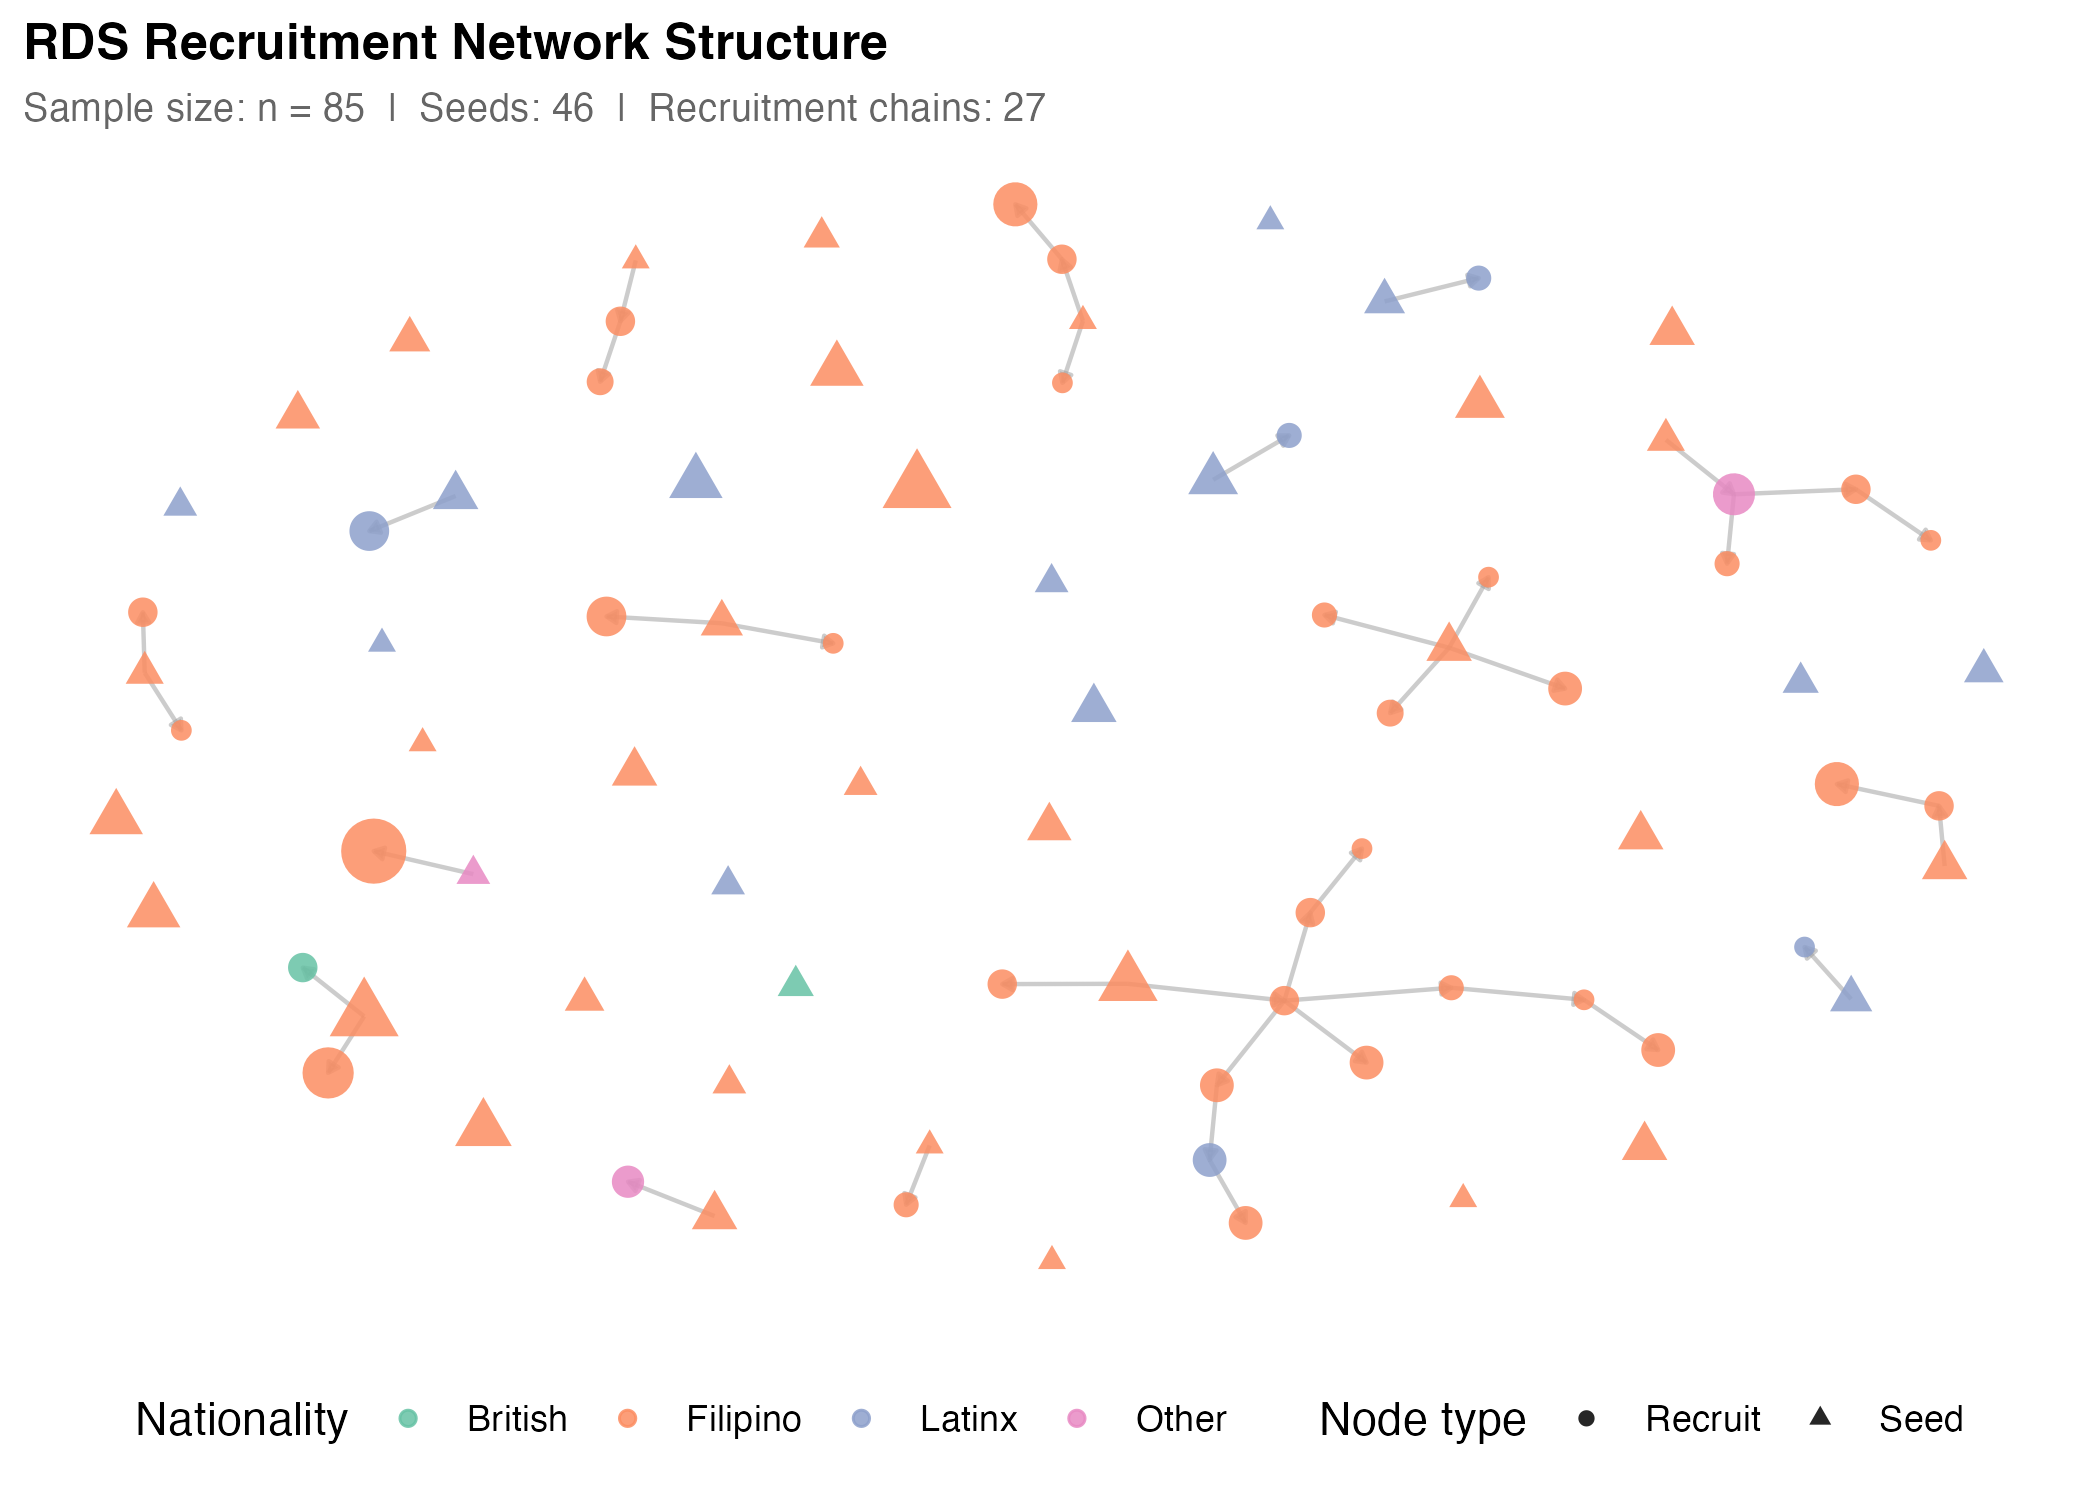
\includegraphics[width=6in,height=\textheight,keepaspectratio]{figures/image1.png}

}

\caption{RDS Recruitment Network Structure. Recruitment chains showing
seed nodes (triangles) and recruit nodes (circles). Node colours
represent nationality clusters; node size is proportional to network
degree. Lines show recruiter-recruit relationships. Source: Authors' own
work.}

\end{figure}%

\begin{longtable}[]{@{}
  >{\raggedright\arraybackslash}p{(\linewidth - 10\tabcolsep) * \real{0.3103}}
  >{\centering\arraybackslash}p{(\linewidth - 10\tabcolsep) * \real{0.1264}}
  >{\centering\arraybackslash}p{(\linewidth - 10\tabcolsep) * \real{0.1264}}
  >{\centering\arraybackslash}p{(\linewidth - 10\tabcolsep) * \real{0.1264}}
  >{\centering\arraybackslash}p{(\linewidth - 10\tabcolsep) * \real{0.1264}}
  >{\centering\arraybackslash}p{(\linewidth - 10\tabcolsep) * \real{0.1379}}@{}}
\caption{Sample composition by nationality cluster and recruitment wave
(n = 85). Wave 0 indicates seed respondents; subsequent waves are
respondent-driven recruits. Filipino respondents dominate the sample
(76\%) and contribute the deepest recruitment chains; other nationality
clusters are smaller and shallower. Source: Authors' own
work.}\tabularnewline
\toprule\noalign{}
\begin{minipage}[b]{\linewidth}\raggedright
Nationality cluster
\end{minipage} & \begin{minipage}[b]{\linewidth}\centering
Wave 0 (seeds)
\end{minipage} & \begin{minipage}[b]{\linewidth}\centering
Wave 1
\end{minipage} & \begin{minipage}[b]{\linewidth}\centering
Wave 2
\end{minipage} & \begin{minipage}[b]{\linewidth}\centering
Wave 3+
\end{minipage} & \begin{minipage}[b]{\linewidth}\centering
Total (n)
\end{minipage} \\
\midrule\noalign{}
\endfirsthead
\toprule\noalign{}
\begin{minipage}[b]{\linewidth}\raggedright
Nationality cluster
\end{minipage} & \begin{minipage}[b]{\linewidth}\centering
Wave 0 (seeds)
\end{minipage} & \begin{minipage}[b]{\linewidth}\centering
Wave 1
\end{minipage} & \begin{minipage}[b]{\linewidth}\centering
Wave 2
\end{minipage} & \begin{minipage}[b]{\linewidth}\centering
Wave 3+
\end{minipage} & \begin{minipage}[b]{\linewidth}\centering
Total (n)
\end{minipage} \\
\midrule\noalign{}
\endhead
\bottomrule\noalign{}
\endlastfoot
Filipino & 35 & 18 & 9 & 3 & 65 \\
Latinx & 4 & 2 & 0 & 0 & 6 \\
British & 2 & 0 & 0 & 0 & 2 \\
Other & 5 & 5 & 2 & 0 & 12 \\
\textbf{Total} & \textbf{46} & \textbf{25} & \textbf{11} & \textbf{3} &
\textbf{85} \\
\end{longtable}

\subsection{3.4 Estimation Framework}\label{estimation-framework}

We analysed the survey sample using multiple estimation models to assess
robustness and conduct sensitivity analyses (see ESM\_2). The dual
structure of our survey instrument---capturing both ego-based and
alter-based network information---enables two fundamentally different
estimation strategies: Respondent-Driven Sampling (RDS) estimators and
Network Scale-Up Methods (NSUM). All analysis code is available at an
anonymised OSF mirror:
\url{https://osf.io/vf5yb/overview?view_only=becc2db3b49c4b258015b648867bf208}.

Before describing each estimator in turn, Table 3 summarises the
information each method uses, the population quantity each method
targets (its \emph{estimand}), and the principal source of
identification risk for each. The four estimators do not target the same
quantity. RDS-SS and MA-RDS estimate own-experience prevalence among the
RDS-reachable population of migrant domestic workers; NSUM estimates
network-visible prevalence among domestic-worker alters as reported by
the respondent; the composite risk index targets the RDS-adjusted mean
severity score. Reading the headline numbers of Section 4 against this
table is essential: the order-of-magnitude RDS--NSUM gap reported there
is in large part a difference of estimand, not a disagreement about a
single underlying quantity (see Section 5.3 for the diagnostic
interpretation).

\begin{longtable}[]{@{}
  >{\raggedright\arraybackslash}p{(\linewidth - 6\tabcolsep) * \real{0.1654}}
  >{\raggedright\arraybackslash}p{(\linewidth - 6\tabcolsep) * \real{0.2481}}
  >{\raggedright\arraybackslash}p{(\linewidth - 6\tabcolsep) * \real{0.2782}}
  >{\raggedright\arraybackslash}p{(\linewidth - 6\tabcolsep) * \real{0.2932}}@{}}
\caption{Estimands and identification vulnerabilities of the four
estimators applied in this paper. Each row characterises one estimator:
what information from the survey it uses, what population quantity it
targets, and what the principal threat to identification is. Source:
Authors' construction.}\tabularnewline
\toprule\noalign{}
\begin{minipage}[b]{\linewidth}\raggedright
Method
\end{minipage} & \begin{minipage}[b]{\linewidth}\raggedright
Information used
\end{minipage} & \begin{minipage}[b]{\linewidth}\raggedright
Estimand
\end{minipage} & \begin{minipage}[b]{\linewidth}\raggedright
Main vulnerability
\end{minipage} \\
\midrule\noalign{}
\endfirsthead
\toprule\noalign{}
\begin{minipage}[b]{\linewidth}\raggedright
Method
\end{minipage} & \begin{minipage}[b]{\linewidth}\raggedright
Information used
\end{minipage} & \begin{minipage}[b]{\linewidth}\raggedright
Estimand
\end{minipage} & \begin{minipage}[b]{\linewidth}\raggedright
Main vulnerability
\end{minipage} \\
\midrule\noalign{}
\endhead
\bottomrule\noalign{}
\endlastfoot
RDS-SS (Section 4.3) & Respondent's own experience + reported degree +
recruitment-chain structure & Own-experience prevalence among the
RDS-reachable population of UK migrant domestic workers & Seed
dependence, shallow recruitment chains, homophily, unobserved degree
heterogeneity \\
MA-RDS (Section 4.4, supporting) & Same as RDS-SS, plus a working
Exponential Random Graph network model conditional on seeds, degree, and
homophily & Model-assisted own-experience prevalence (same target as
RDS-SS but with explicit network structure adjustment) & Network-model
misspecification, convergence limits at small \(n\); does not reliably
converge for continuous outcomes \\
NSUM (MBSU) (Section 4.3, preferred) & Respondent reports about alters
in their personal network & Network-visible prevalence among
domestic-worker alters in the respondents' aggregated network &
Transmission bias, visibility gradient across exploitation behaviours,
alter misclassification, unknown true-positive rate (\(\tau\)) \\
Composite risk index (Section 4.2) & Respondent's own indicator profile
across all eleven ILO indicators & RDS-adjusted population mean of the
formative-additive severity score & Weight specification, construct
validity, formative-vs-reflective measurement assumptions \\
\end{longtable}

To the best of the authors' knowledge, the combined use of both methods
in the same study is rare in peer-reviewed academic research, though it
has appeared in government-funded reports and technical documents from
NGOs and research organizations (IST Research and University of
California, Los Angeles, 2020; Hickman \emph{et al.}, 2025). This paper
contributes to the emerging methodological literature on combining RDS
and NSUM in survey research for hidden populations. We also developed a
novel three-step bootstrap procedure to address uncertainty in NSUM
estimates.

\emph{RDS Estimation:} We implemented three RDS estimators, each with
distinct assumptions: RDS-I (Salganik and Heckathorn, 2004), the
Volz--Heckathorn (VH) estimator (Volz and Heckathorn, 2008), and Gile's
Successive Sampling (RDS-SS) estimator (Gile, 2011). Given our small
sample (85 respondents) and non-negligible sampling fraction, RDS-SS
serves as our primary estimator for binary outcomes because it accounts
for finite population effects. RDS-I, which performs poorly in small
samples and is highly sensitive to seed dependence, is retained as a
historical benchmark.

For continuous outcomes such as the exploitation risk index, we employ
Model-Assisted (MA-RDS) estimators (Gile and Handcock, 2015). MA-RDS is
design-based yet leverages a working Exponential Random Graph Model
(ERGM) with degree and homophily terms to approximate inclusion
probabilities conditional on observed seeds. This approach directly
addresses seed bias and homophily that conventional RDS estimators
cannot correct, accommodates finite-population effects through
successive-sampling logic, and supports valid estimation of both binary
and continuous outcomes. By conditioning on actual seed composition and
subgroup structure, the method reduces bias, improves efficiency, and
provides design-compatible bootstrap uncertainty (Gile, 2011). We note
one important limitation: the MA-RDS implementation in the RDS package
(MA.estimates) is designed primarily for binary traits, and we find that
for the continuous composite risk index it does not converge to a useful
posterior at our sample size (n=85); the credible interval covers
essentially the full support of the variable. We therefore report
frequentist RDS-SS estimates as the headline for the composite index and
reserve MA-RDS estimates for the five binary indicators (see Section 4.2
and ESM\_4).

\emph{Within-Population Scale-Up Estimation (NSUM):} We employ the
Modified Basic Scale-Up (MBSU) model of Feehan and Salganik (2016) in a
non-standard configuration: respondents are themselves members of the
hidden population, reporting on other UK migrant domestic workers they
know. We treat this as a \emph{within-population scale-up} design
(Feehan and Salganik 2016, supplementary materials) or
\emph{alter-report network prevalence} design, estimating
network-visible prevalence among the domestic-worker alters within
respondents' personal networks rather than the hidden-population size.
The estimand differs from the standard NSUM estimand and is documented
in Table 3 above.

The unadjusted MBSU estimator is
\(\hat{p} = \bar{y}_{FH} / \bar{d}_{FF}\) (alter exploitation count
divided by reported network size, averaged over respondents), adjusted
multiplicatively by \(\delta_F\) (degree ratio between hidden and frame
populations) and \(\tau_F\) (true-positive rate; values \(< 1\) capture
under-reporting due to stigma or social distance). Because the frame and
hidden populations coincide here, \(\delta_F\) measures
within-population network-size differences; \(\tau_F\) captures peer-tie
visibility, which is the substantive quantity of interest for the
visibility-gradient diagnostic (Section 5.3).

Our headline NSUM result is the \emph{continuous-\(\tau\) sweep}:
per-indicator prevalence as a function of \(\tau\) over \([0.40, 1.00]\)
in 0.05 increments with \(\delta_F\) fixed at 0.9, with bootstrap 95\%
CIs at each value (ESM\_4 Figure 1). For comparison with the
discrete-tier NSUM literature (Killworth et al.~1998; Maltiel et
al.~2015; Feehan and Salganik 2016), we report three reference scenarios
--- Unadjusted (\(\delta = 1.0, \tau = 1.0\)), Moderate
(\(\delta = 0.9, \tau = 0.85\)), Conservative
(\(\delta = 0.8, \tau = 0.70\)) --- as discrete points on the continuous
curve.

\subsection{3.5 Comparative Rationale: Ego-Based vs.~Alter-Based
Inference}\label{comparative-rationale-ego-based-vs.-alter-based-inference}

RDS and NSUM both exploit social network structures but use
fundamentally different information for inference. RDS uses ego-based
information: respondents report their own characteristics and network
degree, which are combined with recruitment wave to adjust for unequal
inclusion probabilities. The underlying logic is that individuals with
larger networks are more likely to be recruited, creating bias toward
highly connected respondents. RDS estimators explicitly correct for this
by weighting observations according to network degree and recruitment
path.

NSUM uses alter-based information -- respondents serve as informants
about the wider hidden population, reporting how many people they know
with specific traits. These reports are scaled up using assumptions
about network size and visibility to infer prevalence in the broader
population. NSUM does not depend on recruitment chains but instead on
the accuracy of respondents' knowledge about others in their social
circles.

Applying both methods to the same dataset allows for triangulation
across two fundamentally different inferential logics---one anchored in
``who recruited whom'' (RDS), the other in ``how many alters fit this
category'' (NSUM).

\textbf{3.6 Choice of population size and the invariance of prevalence.}
Prevalence estimates reported throughout the paper are invariant to the
assumed UK domestic-worker population size \(N\) in the asymptotic
regime in which \(n/N\) is small. RDS-I, RDS-II/Volz-Heckathorn, and the
MBSU NSUM prevalence formulas are algebraically free of \(N\); RDS-SS
and MA-RDS contain \(N\) only through finite-population corrections
whose magnitude scales with \(n/N\). At \(n = 85\) our sampling fraction
is at most 0.17\% (for \(N = 50{,}000\)) and as low as 0.005\% (for
\(N = 1{,}740{,}000\)), all well below the conventional 5\% threshold at
which finite-population corrections become non-negligible. Headline
estimates use \(N = 980{,}000\) (the EU baseline); the MA-RDS Bayesian
analysis uses \(N = 50{,}000\) for computational tractability. Cached
estimates across all four values agree to within bootstrap noise; full
algebraic derivation and empirical confirmation are in ESM\_4 Section A
(Population Size and the Invariance of Prevalence).

\subsection{3.7 Bootstrap and Sensitivity
Procedures}\label{bootstrap-and-sensitivity-procedures}

To appropriately characterise uncertainty in NSUM estimates, we
implement a three-step bootstrap procedure. This approach resamples
respondents, their reported alters, and the exploitation classifications
simultaneously, thereby capturing uncertainty at each stage of the
inference process. This procedure provides more realistic confidence
intervals than those generated by conventional variance estimators,
particularly for small samples such as ours. Details of the bootstrap
implementation and diagnostic checks are provided in Online Resource
ESM\_3. Several of the estimation procedures implemented here adopt
Bayesian or model-assisted frameworks, which are particularly
appropriate for modest sample sizes because they incorporate uncertainty
directly into the estimation process (Gile et al., 2018). Our custom
neighbourhood bootstrap procedure similarly quantifies uncertainty by
repeatedly resampling ego and alter information, producing empirically
grounded confidence intervals rather than relying on asymptotic
approximations that assume large samples.

For RDS estimators, we employ neighborhood bootstrap methods that
preserve the network structure while resampling (Yauck \emph{et al.},
2022). Sensitivity analyses examine robustness to population size
assumptions (50K, 100K, 980K, 1.74M) and NSUM adjustment factor values.
Full results are reported in Online Resource ESM\_4.

\section{Results}\label{results}

We present results in five subsections. Section 4.1 describes the
analytical sample. Sections 4.2 and 4.3 report the preferred prevalence
estimates for the continuous composite risk index and the five binary
ILO-aligned indicators respectively. For binary indicators, the
preferred estimator is RDS-SS (Gile's Successive Sampling) with
neighbourhood-bootstrap 95\% confidence intervals; for the composite
risk index, also RDS-SS, because the Bayesian Model-Assisted estimator
does not converge to a useful posterior on continuous outcomes at our
sample size (Section 3.4). The preferred NSUM result is the
continuous-\(\tau\) sweep over \(\tau \in [0.40, 1.00]\) with \(\delta\)
fixed at 0.9 (Section 3.4; ESM\_4 Figure 1); the Moderate discrete-tier
point estimate (\(\delta = 0.9\), \(\tau = 0.85\)) is reported alongside
as a reference scenario for direct comparison with the discrete-tier
NSUM literature. Section 4.4 reports supporting estimates --- Bayesian
Model-Assisted estimates for the five binary indicators, alternative RDS
estimators (RDS-I, RDS-II), and NSUM under alternative adjustment-factor
scenarios --- included for comparison and to support the robustness
claims in Section 4.5. Section 4.5 summarises the sensitivity analyses,
with full details in ESM\_4.

A scope note before the numbers. The estimates reported below are
exploratory population-adjusted estimates for the RDS-reachable
population of UK migrant domestic workers connected to the participating
civil-society networks (primarily Kalayaan and the Latin American
Women's Rights Service). They should not be read as definitive national
prevalence figures for all UK migrant domestic workers. The four
estimators target different population quantities (Section 3.4, Table
3), so absolute levels also differ by estimator in interpretable ways.

\subsection{4.1 Descriptive Overview}\label{descriptive-overview}

Sample characteristics are presented in Table 2 and Figure 1. 97
respondents completed the survey; 85 with non-zero network degree were
included in RDS analysis. The analytical sample is 93\% transnational
migrant, 97\% female, 76\% Filipino, with over half aged 45+ and 45\%
self-employed.

\subsubsection{4.1.1 RDS Sampling
Diagnostics}\label{rds-sampling-diagnostics}

Because the RDS estimators reported below rely on assumptions about
chain propagation, degree homogeneity within seed groups, and reaching
equilibrium across recruitment waves, we report the key sampling
diagnostics here in the main text rather than in the supplement. The
diagnostics are summarised in Table 4 and visualised in Figure 2; Figure
1 (above) shows the full recruitment graph.

\begin{longtable}[]{@{}
  >{\raggedright\arraybackslash}p{(\linewidth - 4\tabcolsep) * \real{0.4434}}
  >{\centering\arraybackslash}p{(\linewidth - 4\tabcolsep) * \real{0.1415}}
  >{\raggedright\arraybackslash}p{(\linewidth - 4\tabcolsep) * \real{0.4057}}@{}}
\caption{RDS sampling diagnostics for the analytical sample (n = 85).
Computed directly from \texttt{data/processed/data\_nonzero.csv}; see
Section 4.1.1 below and ESM\_4 (convergence plots per indicator) for the
full set. Source: Authors' construction.}\tabularnewline
\toprule\noalign{}
\begin{minipage}[b]{\linewidth}\raggedright
Diagnostic
\end{minipage} & \begin{minipage}[b]{\linewidth}\centering
Value
\end{minipage} & \begin{minipage}[b]{\linewidth}\raggedright
Interpretation
\end{minipage} \\
\midrule\noalign{}
\endfirsthead
\toprule\noalign{}
\begin{minipage}[b]{\linewidth}\raggedright
Diagnostic
\end{minipage} & \begin{minipage}[b]{\linewidth}\centering
Value
\end{minipage} & \begin{minipage}[b]{\linewidth}\raggedright
Interpretation
\end{minipage} \\
\midrule\noalign{}
\endhead
\bottomrule\noalign{}
\endlastfoot
Total respondents (analytical sample) & 85 & non-zero network degree \\
Seeds (recruiter.id == -1) & 46 (54\%) & majority of sample is
seed-recruited \\
Recruits (wave 1+) & 39 (46\%) & sourced via respondent-driven
referral \\
Active recruitment chains (length \(\geq 2\)) & 16 & seeds that
recruited at least once \\
Singleton seeds (chain length = 1) & 30 & seeds with no successful
recruits \\
Maximum chain length & 12 & one dominant chain (seed \#55) drives much
of the wave depth \\
Maximum wave depth & 4 & shallow relative to RDS conventions (5--6 waves
typical for equilibrium) \\
Respondents at wave \(\geq 3\) & 6 (7\%) & only 7\% reached the depth at
which RDS equilibrium typically obtains \\
Median reported network size (q13) & 5 & half of respondents report
knowing \(\leq 5\) other domestic workers \\
Mean reported network size & 8.9 & mean inflated by a long right tail
(max = 105); strong degree skew \\
Largest nationality cluster & Filipino (n = 65) & 76\% of n = 85;
homophily by nationality within chains is consequently high \\
\end{longtable}

\begin{figure}[H]

{\centering 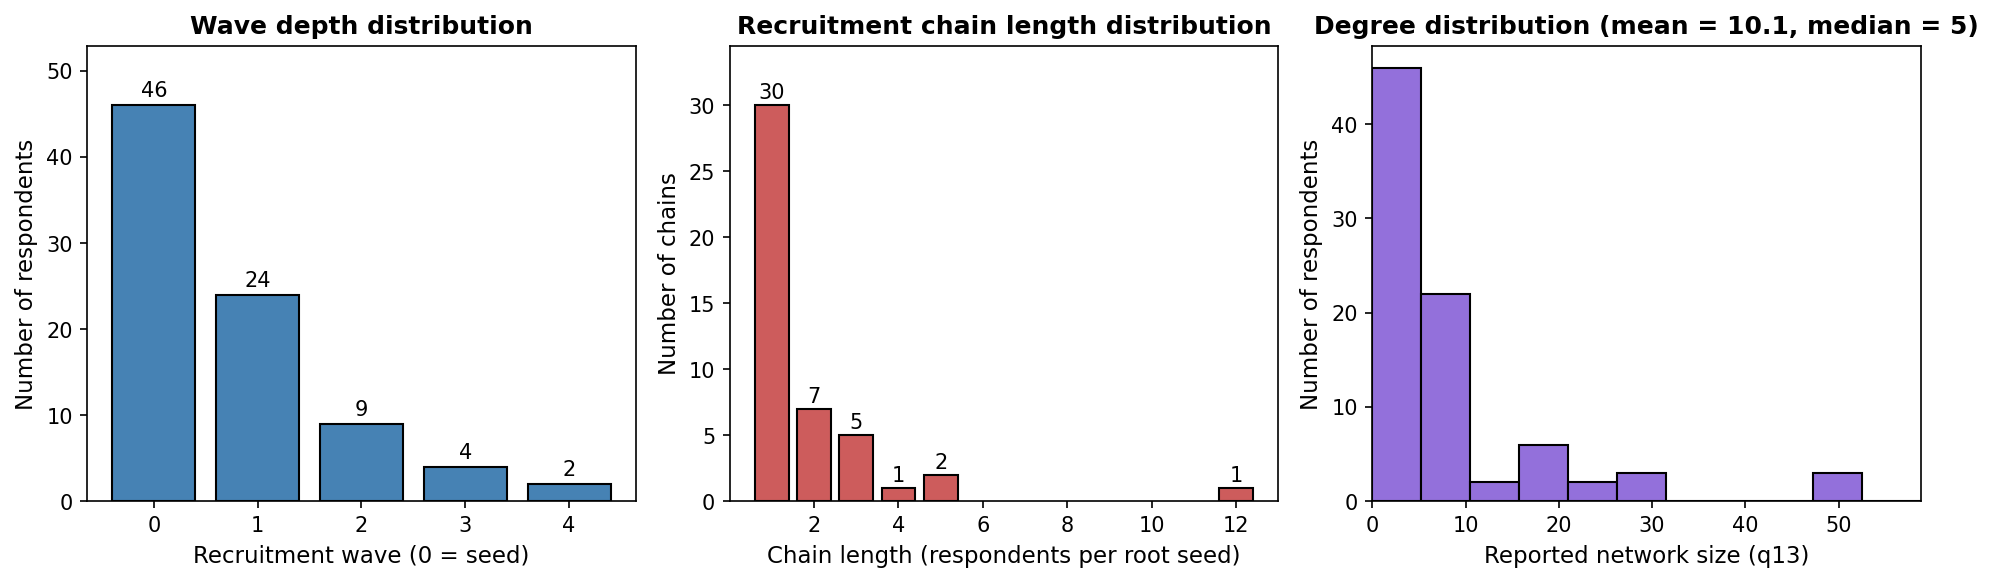
\includegraphics[width=6in,height=\textheight,keepaspectratio]{figures/rds_diagnostics.png}

}

\caption{RDS sampling-design diagnostics. Left: distribution of
respondents by recruitment wave; majority are seeds (wave 0) with only 6
of 85 respondents reaching wave 3 or higher. Middle: distribution of
recruitment-chain lengths by root seed; 30 of 46 chains are singletons
(seed with no recruits), and one chain (seed \#55, length 12) accounts
for a disproportionate share of wave-2+ respondents. Right: distribution
of reported network size (q13), showing strong right skew (median 5,
mean 8.9, max 105). Source: Authors' construction from
\texttt{data/processed/data\_nonzero.csv}.}

\end{figure}%

Three features warrant acknowledgement. The high share of seeds (54\%)
and low share of wave-3+ respondents (7\%) mean the sample is closer to
a \emph{civil-society-mediated web-RDS sample with network adjustment}
than to a fully propagated RDS sample; the standard RDS assumption of
approximately stationary sampling distribution is therefore only
partially satisfied. The chain-length distribution is also highly
skewed: one chain (seed \#55, length 12) accounts for roughly a third of
wave-2+ respondents, and a leave-one-out sensitivity excluding that
chain (ESM\_4) shifts headline binary prevalences by 2--6 percentage
points without changing the indicator ordering. Finally, with 76\% of
the sample Filipino, most chains are within-Filipino, so prevalence
estimates are best read as estimates for the Filipino-dominated
civil-society-reachable subpopulation rather than for all UK migrant
domestic workers. The practical implication for the headline numbers is
that RDS-SS, MA-RDS, and the composite index should all be read with
this constrained sampling structure in view; the RDS-I vs RDS-SS
comparison reported in Section 4.4 quantifies how much the standard
equilibrium assumption matters (RDS-I runs 5--15 percentage points
higher, with the gap larger where seed-cluster homophily is strongest).

\subsection{4.2 Continuous Risk Index: RDS-SS
Estimates}\label{continuous-risk-index-rds-ss-estimates}

One of the central contributions of this study is the introduction of a
continuous risk index measuring degree of exposure to labour
exploitation. The index is constructed from all eleven ILO indicators of
forced labour, with sub-weights anchored on the ILO medium/strong
severity gradation: strong-indicator categories (intimidation and
threats, physical and sexual violence, retention of identity documents)
receive larger sub-weights than medium-indicator categories.
NRM-referral history and payment below the national living wage are
reported as separate binary evidentiary flags and are not part of the
composite (Section 3.2, Table 1; full per-category weights in ESM\_1,
Table 1). Rather than treating exploitation as a dichotomy, the risk
index conceptualises every domestic worker as facing some degree of
potential exploitation, varying continuously in intensity from low to
high.

The preferred population-adjusted estimate uses Gile's Successive
Sampling (RDS-SS) Horvitz-Thompson estimator with neighbourhood
bootstrap. The estimated mean risk index for the RDS-reachable
population of UK migrant domestic workers connected to the participating
civil-society networks is 37.0\% of the theoretical maximum (95\% CI
30.9--44.0\%), very close to the observed sample mean of 37.5\% ---
indicating that the RDS-SS finite-population adjustment makes only a
small correction at our sampling fraction. We report RDS-SS rather than
the Bayesian Model-Assisted estimator for the composite index because,
as noted in Section 3.4, MA-RDS does not converge to a useful posterior
on continuous traits at this sample size; for completeness Figure 2
shows the MA estimate alongside the RDS-SS and sample estimates, with
the wide MA credible interval making the limitation visible.

\begin{figure}[H]

{\centering 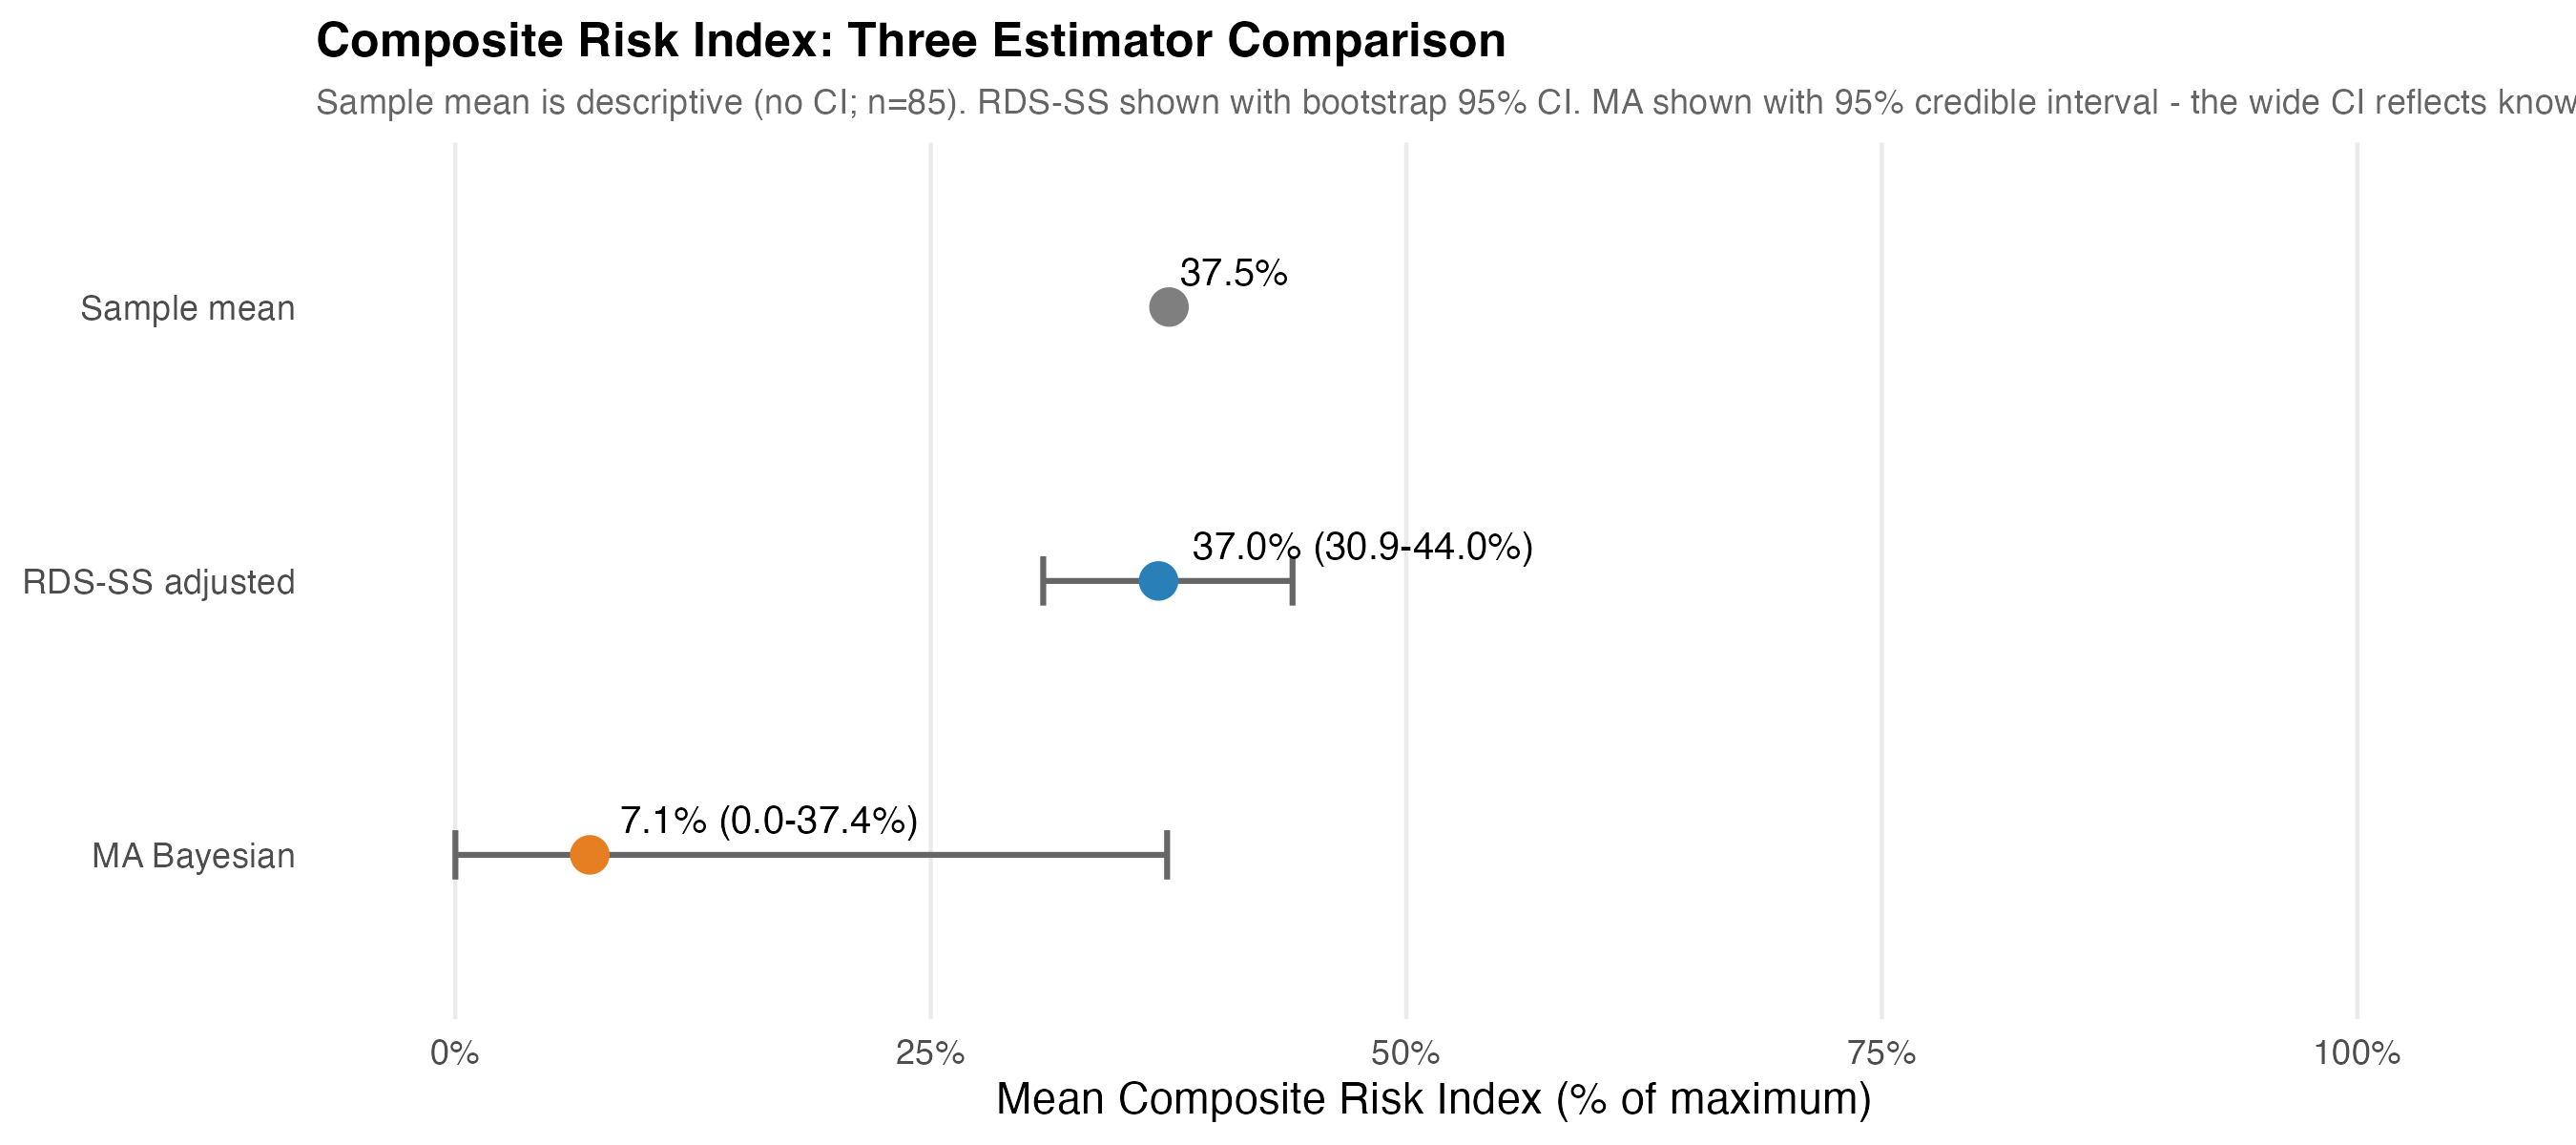
\includegraphics[width=6in,height=\textheight,keepaspectratio]{figures/image3.png}

}

\caption{Composite Risk Index: Comparison of Three Estimators. Mean
composite risk index across the observed RDS sample (descriptive; n=85),
the RDS-SS adjusted estimator (Gile's Successive Sampling with bootstrap
95\% CI), and the Bayesian Model-Assisted (MA) estimator (with 95\%
credible interval). The wide MA credible interval reflects known
limitations of model-assisted inference for continuous outcomes; the
RDS-SS estimate is the more reliable population-adjusted figure. Source:
Authors' own work.}

\end{figure}%

\subsection{4.3 Binary Exploitation Indicators: Preferred Prevalence
Estimates}\label{binary-exploitation-indicators-preferred-prevalence-estimates}

Table 5 reports the preferred prevalence estimates for each of the five
binary ILO-aligned indicators in the RDS-reachable population,
presenting RDS-SS (ego-based) and MBSU NSUM Moderate (alter-based)
estimates side by side. ESM\_4 Figure B.1 shows the RDS-SS estimates
with per-method bootstrap CIs for visual comparison with the RDS-I
estimator (the preferred binary-indicator estimator is RDS-SS).

Prevalence is high for most indicators in this hidden population. RDS-SS
estimates range from 35.4\% for document withholding to 84.2\% for
excessive working hours; MBSU Moderate NSUM estimates range from 1.08\%
(document withholding) to 2.98\% (excessive hours). The
order-of-magnitude difference between RDS and NSUM is consistent with a
visibility gradient: ego-based RDS reports capture what the respondent
personally experienced, alter-based NSUM reports capture what other
domestic workers can see. For behaviours that occur behind closed doors,
the gap between own-experience and network-visible reports is large, and
the divergence between RDS and NSUM estimates is correspondingly large
(Section 5.3 develops the diagnostic interpretation in detail; the gap
also reflects differences in estimand, sampling frame, transmission
bias, and the unknown true-positive rate). Within methods, the ordering
of indicators by prevalence is remarkably stable: excessive working
hours consistently the highest, followed by threats and abuse and
pay-related issues, with document withholding the lowest. This
consistency across methods, even where absolute levels differ, is a
robustness signal for the indicator hierarchy itself.

\begin{longtable}[]{@{}
  >{\raggedright\arraybackslash}p{(\linewidth - 4\tabcolsep) * \real{0.3086}}
  >{\raggedright\arraybackslash}p{(\linewidth - 4\tabcolsep) * \real{0.2593}}
  >{\raggedright\arraybackslash}p{(\linewidth - 4\tabcolsep) * \real{0.4321}}@{}}
\toprule\noalign{}
\begin{minipage}[b]{\linewidth}\raggedright
\textbf{Indicator}
\end{minipage} & \begin{minipage}[b]{\linewidth}\raggedright
\textbf{RDS-SS (95\% CI)}
\end{minipage} & \begin{minipage}[b]{\linewidth}\raggedright
\textbf{MBSU NSUM (Moderate) (95\% CI)}
\end{minipage} \\
\midrule\noalign{}
\endhead
\bottomrule\noalign{}
\endlastfoot
Document withholding & 35.4\% (21.1--49.8\%) & 1.08\% (0.30--3.13\%) \\
Threats and abuse & 56.9\% (42.3--72.1\%) & 2.69\% (1.86--5.86\%) \\
Pay-related issues & 51.6\% (36.5--65.5\%) & 2.88\% (1.90--5.68\%) \\
Excessive working hours & 84.2\% (72.2--93.6\%) & 2.98\%
(1.84--5.51\%) \\
Limited access to help & 60.6\% (45.2--74.1\%) & 2.03\%
(0.67--4.88\%) \\
\end{longtable}

\begin{figure}[H]

{\centering 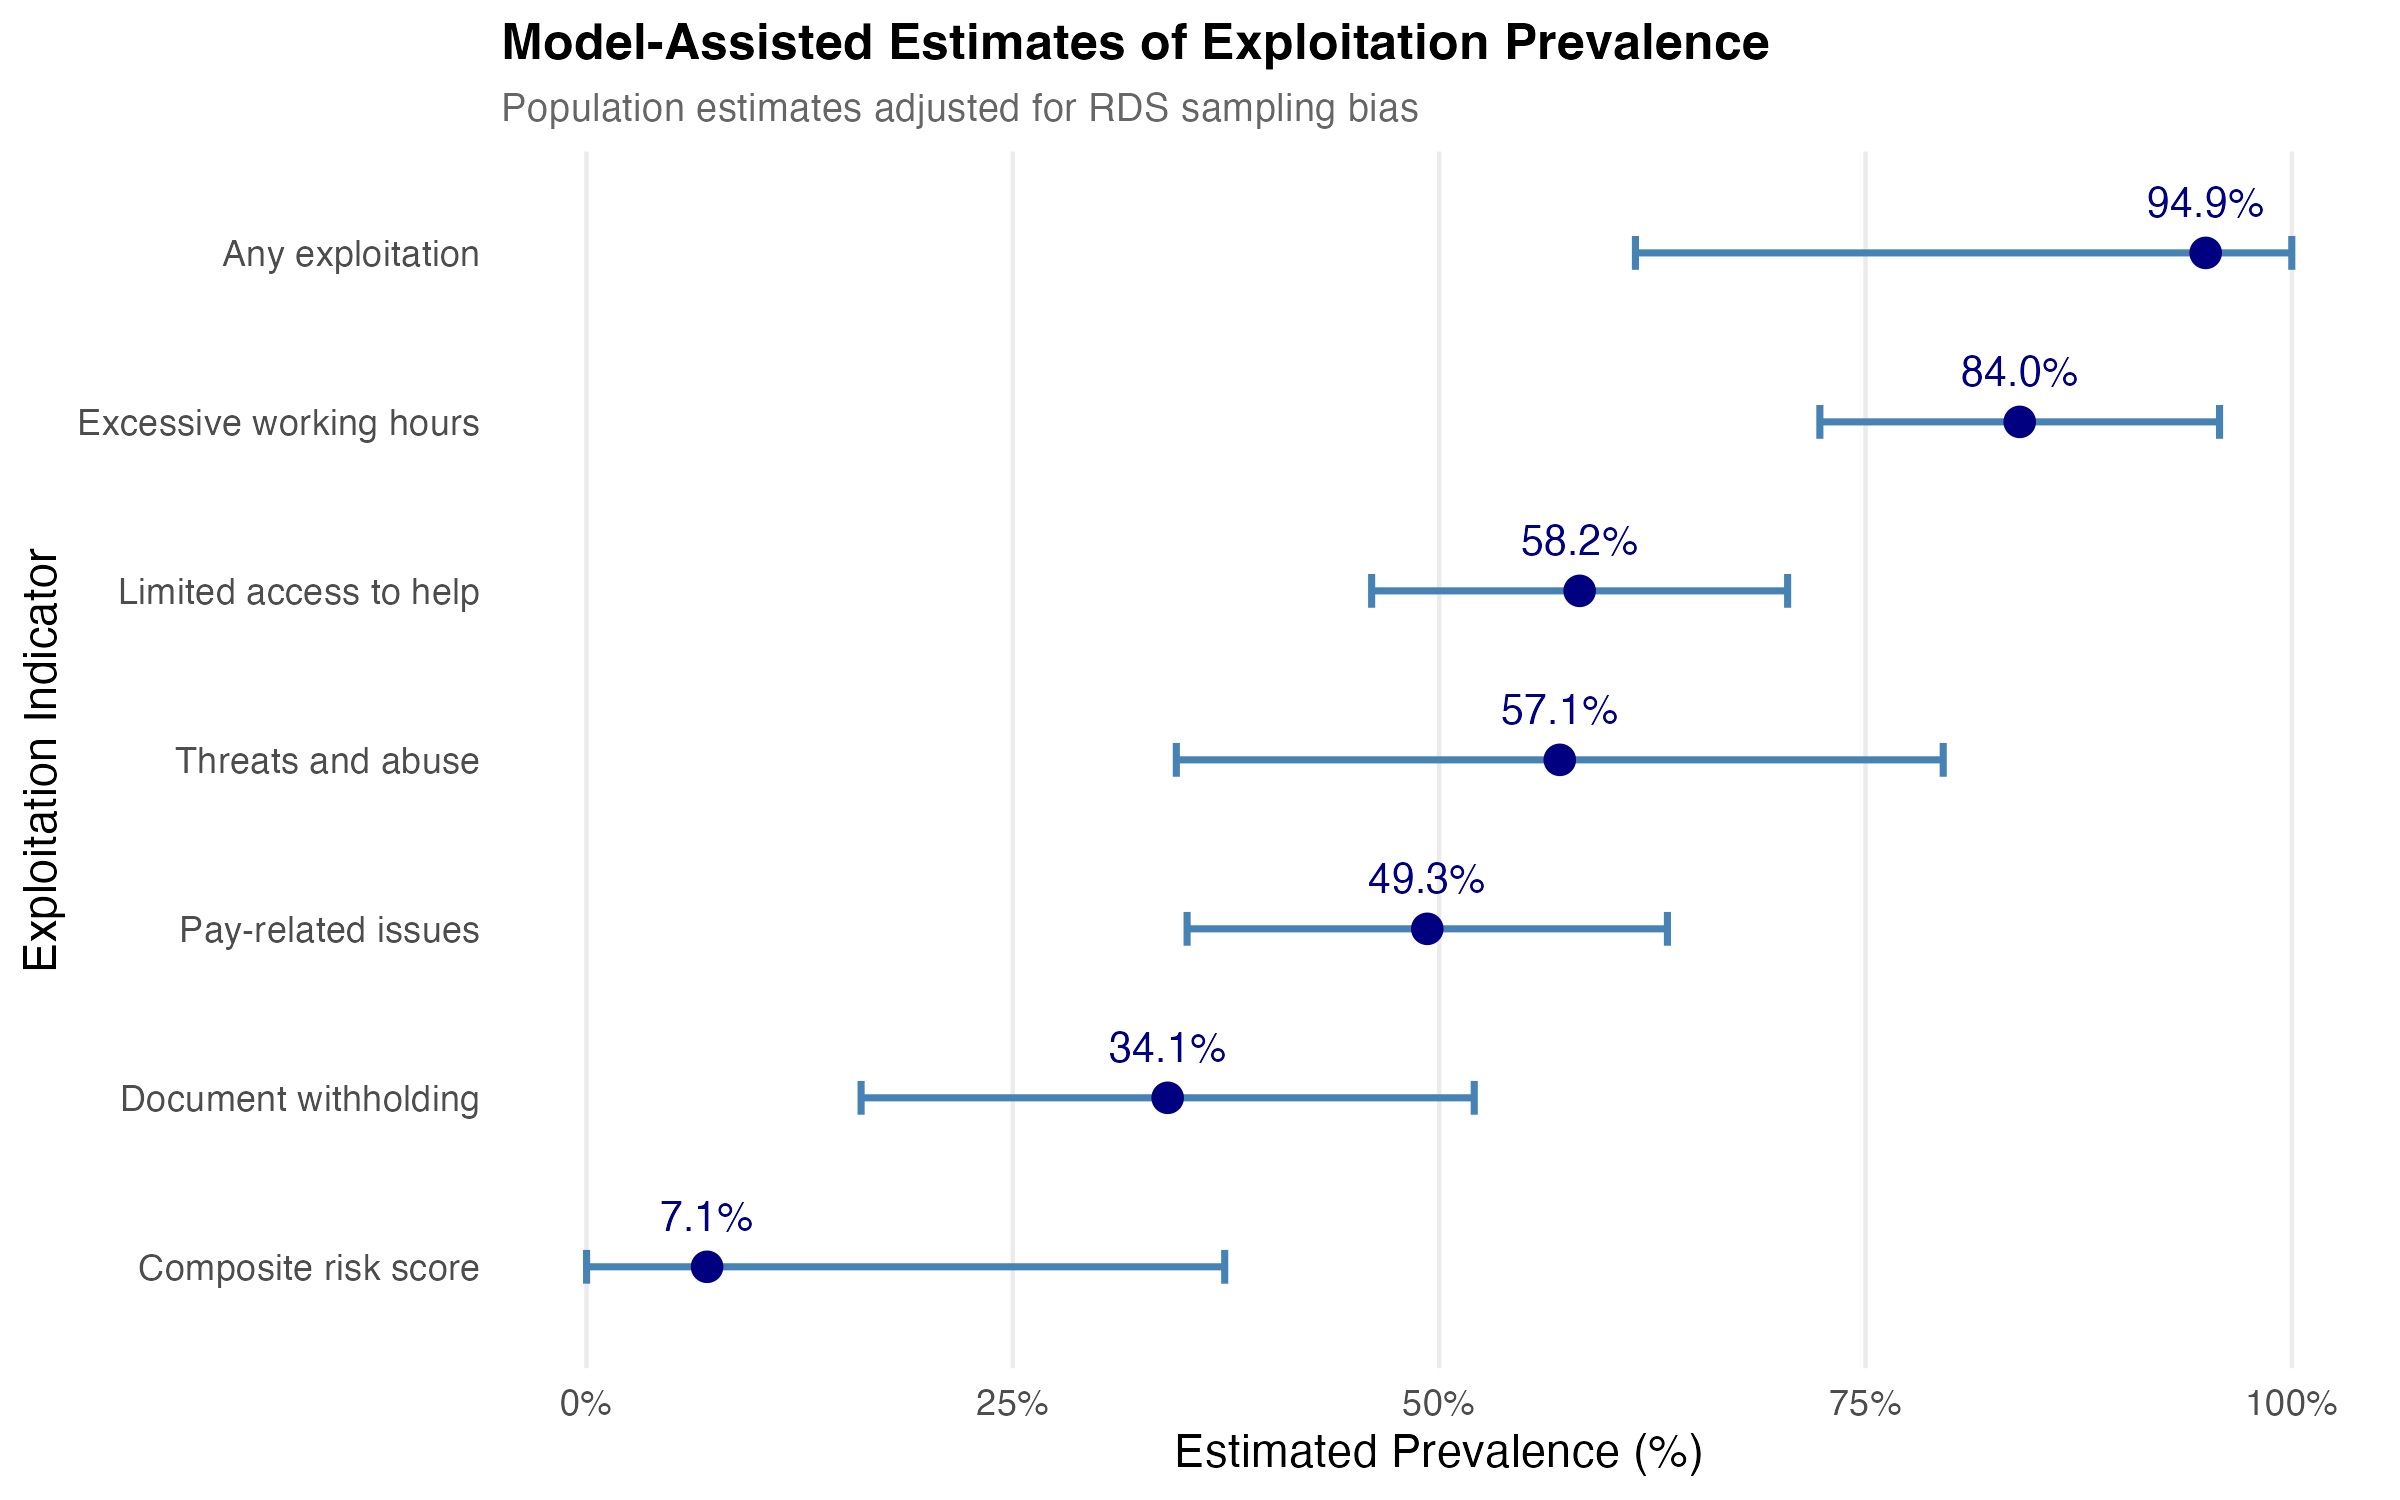
\includegraphics[width=6in,height=\textheight,keepaspectratio]{figures/image4.png}

}

\caption{Model-Assisted Estimates of Exploitation Prevalence. Population
prevalence estimates with 95\% credible intervals for each exploitation
indicator, ordered by prevalence magnitude. Posterior intervals are from
Bayesian Model-Assisted inference (Gile \& Handcock, 2015) at N=50,000
with seed.selection=`degree'. Source: Authors' own work.}

\end{figure}%

\subsection{4.4 Supporting Estimates and Method
Comparison}\label{supporting-estimates-and-method-comparison}

Three additional families of estimates are reported in full in ESM\_4
Section B (Supporting Estimates and Method Comparison) for transparency
and robustness: (a) Bayesian Model-Assisted estimates (MA-RDS) of the
five binary indicators at \(N = 50{,}000\) with 95\% credible intervals
(ESM\_4 Table 3); posterior means range from 34.1\% (document
withholding) to 84.0\% (excessive working hours) and substantively
replicate the RDS-SS ordering reported in Table 5. (b) Direct comparison
of RDS-I and RDS-SS estimators for each indicator with per-method
bootstrap 95\% CIs (ESM\_4 Table 4); RDS-I runs systematically higher
than RDS-SS by 5--15 percentage points, consistent with the standard
finding that RDS-I is sensitive to seed dependence and performs poorly
at the small sample sizes and shallow chain depths characteristic of our
design (Section 4.1.1). (c) NSUM under the three discrete
adjustment-factor tiers (Unadjusted, Moderate, Conservative; ESM\_4
Table 5), presented for direct comparison with the discrete-tier NSUM
literature. The substantive headline NSUM result is the
continuous-\(\tau\) sweep reported in Section 4.5.

\subsection{4.5 Sensitivity and
Robustness}\label{sensitivity-and-robustness}

Three sensitivity analyses are reported in full in ESM\_4. First, the
continuous-\(\tau\) NSUM sweep (ESM\_4 Figure 1) shows MBSU prevalence
monotonically increasing as \(\tau\) decreases; the increase is modest
across the plausible range \(\tau \in [0.7, 1.0]\) and substantial only
at low \(\tau \le 0.5\). This continuous picture supersedes the
discrete-tier comparison (Section 4.4) for substantive inference about
how visibility assumptions affect estimates.

Second, the MA-RDS seed-selection sensitivity (ESM\_4 Figure 2) shows
that the Bayesian MA posterior estimates are insensitive to the choice
of seed-selection method (degree, random, sample) at our sample size ---
different chains converge to the same posterior, confirming model
robustness to initialisation.

Third, cross-indicator and cross-method consistency: across the five
indicators and the four main estimators (RDS-I, RDS-SS, MA-RDS, MBSU
NSUM Moderate), the rank-ordering of indicators by prevalence is stable.
Excessive working hours is consistently highest, followed by threats and
abuse and pay-related issues, with document withholding the lowest.
Absolute prevalence levels vary by method but the substantive picture
--- which exploitation behaviours are most common, which least --- does
not.

\section{Discussion}\label{discussion}

\subsection{5.1 Summary of Findings}\label{summary-of-findings}

Across five ILO-aligned binary indicators measured on a
respondent-driven sample of 85 UK migrant domestic workers, RDS-SS
Horvitz-Thompson prevalence estimates range from 35.4\% for document
withholding (95\% CI 21.1--49.8\%) to 84.2\% for excessive working hours
(95\% CI 72.2--93.6\%); a composite continuous risk index covering all
eleven indicator dimensions gives an estimated mean exploitation
intensity of 37.0\% (95\% CI 30.9--44.0\%). MBSU Moderate NSUM estimates
of the same five binary indicators range from 1.08\% (document
withholding) to 2.98\% (excessive hours), an order-of-magnitude lower
than the RDS-SS figures. The within-method ordering of indicators is
consistent across methods: excessive working hours always highest,
followed by threats and abuse and pay-related issues, with document
withholding always lowest. This consistency, alongside the
order-of-magnitude gap between ego-based (RDS) and alter-based (NSUM)
estimates, is the central empirical finding of the paper. The remainder
of this section interprets both the absolute estimates and the
inter-method divergence.

\subsection{5.2 Methodological Reflections and
Contributions}\label{methodological-reflections-and-contributions}

This paper makes two contributions to the measurement of modern slavery
among hidden populations. First, we apply RDS and NSUM to the same
matched survey instrument in what is, to our knowledge, among the first
applications of this dual design in any developed-economy setting for
the measurement of forced-labour and modern-slavery indicators; the
design supports direct comparison of ego-based and alter-based estimates
on a like-for-like indicator set without claiming they target the same
population quantity (Section 3.4, Table 3). Second, we operationalise
modern slavery as a graded latent construct rather than a binary
condition, supporting both indicator-level prevalence estimates and an
eleven-indicator formative additive composite risk index for ordinal
severity gradation.

The combined contributions are: (i) operationalising exploitation both
as a five-indicator binary set (Section 4.3) and as a formative additive
composite spanning all eleven ILO categories (Section 4.2); (ii)
applying RDS and NSUM to the same instrument, exposing the visibility
gradient where the two methods diverge (Section 5.3); (iii) implementing
a three-step bootstrap procedure for NSUM that resamples respondents,
alters, and exploitation classifications in succession; and (iv)
demonstrating feasibility in a stigmatised and under-researched
population mediated by civil-society partners, with the methodology
generalisable to other hidden populations relevant to SDG 8.7 monitoring
(Section 5.6).

\subsection{5.3 The RDS--NSUM Divergence as
Diagnostic}\label{the-rdsnsum-divergence-as-diagnostic}

Two related concerns are taken up here: that the reported prevalence
estimates span a wide range, and that the sample size (n = 85) is small
for population-level inference. We argue that the apparent ``wide
range'' in fact reflects three conceptually distinct sources of
dispersion, each of which carries a different epistemic status; and that
on the only one of the three sources where sample size matters, n = 85
is competitive for hidden-population designs and the per-method
bootstrap confidence intervals we now report propagate the implied
uncertainty honestly.

The ``wide range'' concern conflates three distinct sources of
dispersion in the reported numbers. We should not treat them as a single
undifferentiated band of uncertainty. The first source is
across-indicator variation. Within any single method, prevalence varies
substantially across the five ILO-aligned indicators --- under RDS-SS,
from 35.4\% for document withholding to 84.2\% for excessive working
hours, a 49-percentage-point spread. This is a substantive finding, not
noise. It tells us that severe forms of coercion (document confiscation,
which the ILO classifies as a strong indicator any one of which alone is
sufficient to indicate forced labour) are less common in this population
than less severe forms of abuse (excessive hours, an ILO medium
indicator whose presence individually is suggestive but not definitive).
The hierarchy is interpretable, matches the ILO severity gradation, and
is reproduced across methods. Collapsing this hierarchy into a single
``wide range'' headline obscures what is arguably the paper's most
policy-relevant finding: that different exploitation behaviours have
meaningfully different population frequencies.

The second source is across-method variation. For any single indicator,
RDS and NSUM estimates differ by roughly an order of magnitude: document
withholding sits at 35.4\% under RDS-SS but at 1.08\% under MBSU
Moderate NSUM; excessive hours at 84.2\% versus 2.98\%. This too is a
substantive finding, not noise. It is the visibility gradient diagnostic
that lies at the centre of this paper's contribution: ego-based RDS asks
what happened to you, alter-based NSUM asks what you can see happening
to others, and the two answer related but different questions for
behaviours that occur behind closed doors --- almost by definition for
domestic work conducted inside a private home. The order-of-magnitude
gap between our RDS and NSUM estimates is therefore not a methodological
pathology to be reconciled. The gap is consistent with a visibility
gradient: some exploitation behaviours are readily observable by peers,
whereas others remain concealed within the household. We are cautious
not to claim that the gap \emph{quantifies} visibility, however, because
the divergence also reflects differences in estimand (own-experience
versus network-visible prevalence, Section 3.4 Table 3), differences in
sampling frame, transmission bias, and the unknown true-positive rate
\(\tau\) (which the continuous-\(\tau\) sweep in ESM\_4 makes explicit).
Reporting RDS and NSUM side-by-side (Table 5) is the paper's design
choice precisely because the gap is interpretable as diagnostic evidence
rather than as a single estimate of a single quantity.

The third source --- and the only one that is irreducibly statistical
uncertainty in the conventional sense --- is within-method,
within-indicator sampling variation. This is what the bootstrap
confidence intervals capture, and these are much tighter than the
across-indicator and across-method spreads taken together. RDS-SS
within-indicator CIs span 21--30 percentage points; MBSU Moderate
within-indicator CIs span 1--4 percentage points. A residual component
of within-method uncertainty for NSUM specifically comes from the
unknown true-positive rate \(\tau\), which the continuous-\(\tau\) sweep
across \(\tau \in [0.40, 1.00]\) in ESM\_4 reports as a sensitivity
curve rather than committing to a single point estimate. Sample-size
effects operate through this third channel and only this third channel:
more respondents would narrow the bootstrap CIs but would not narrow the
across-indicator hierarchy (which is real) or the across-method gap
(which is the diagnostic finding).

Three further observations support the visibility-gradient
interpretation. The gap is largest for indicators we would expect to be
least visible (document withholding, concealed by definition: ego/alter
ratio 33\(\times\)) and smaller for more visible indicators (excessive
working hours: ratio 28\(\times\)). The within-method ordering of
indicators is stable across methodologically unrelated estimators --- a
robustness signal that justifies treating the indicators as distinct
gradations of severity even where absolute levels differ. And the
direction of the bias matches the NSUM transmission-bias literature
(Feehan and Salganik 2016; Maltiel et al.~2015; Killworth et al.~1998),
which documents systematic alter under-reporting for stigmatised traits,
often of an order of magnitude.

On sample size: n = 85 is small by household-survey standards but
competitive for hidden-population studies (published RDS applications
operate at 100--300; UK domestic-worker NGO samples are typically
smaller and not network-recruited). The dual ego/alter survey design
also extracts more information per respondent than a household survey,
yielding 170 indicator measurements per ILO category once both reports
are counted before any network-weighting amplification. Chain depth is
shallower than the RDS design envisaged (Section 4.1.1); a longer field
period would help in future replications.

\subsection{5.4 Generalisability and Indicator
Coverage}\label{generalisability-and-indicator-coverage}

One may reasonably question whether estimates from a single
civil-society-mediated sample can support population-level claims, and
whether the five indicators we measure capture the full ILO conceptual
space. Both are valid concerns and both warrant qualification of the
paper's claims rather than retreat from them.

On generalisability: the sample is drawn from two London-based
civil-society networks (Kalayaan and the Latin American Women's Rights
Service) and is not representative of all UK migrant domestic workers,
much less all hidden populations relevant to SDG 8.7. Demographics skew
Filipino and Latinx, omitting substantial South Asian, East African, and
Eastern European communities not reached by the participating networks.
What the paper demonstrates is methodological feasibility on a hard
realistic case and a set of specific estimates for that sample; the
methodology generalises but the specific prevalence numbers should not
be extrapolated beyond this sample.

On indicator coverage: we measure five ILO indicators directly as binary
prevalences, jointly covering nine of the eleven ILO indicators (Section
3.2, Table 1). The remaining two --- abuse of vulnerability and
deception --- require retrospective interpretation that brief-survey
self-report cannot reliably elicit at \(n = 85\); both are retained in
the composite risk index (ESM\_1, Categories 1 and 2). The paper's claim
is therefore not ``prevalence of forced labour as defined by the eleven
ILO indicators'' but ``prevalence of nine of the eleven as direct binary
measures, with the remaining two captured through the composite only''.

Taking the divergence diagnostic, the generalisability qualifications,
and the indicator coverage qualifications together, what does this
design licence the paper to claim? Not a single point estimate of ``the
prevalence of forced labour among UK domestic workers'', because no
single point estimate is identified. If RDS over-samples respondents
with first-hand experience of exploitation and NSUM systematically
under-detects exploitation concealed behind closed doors, then the true
population prevalence for any given indicator likely lies somewhere
between the two reports --- but the location on that interval depends on
assumptions about visibility, sampling, and reporting that the data
cannot fully pin down. We treat this as an interpretive working
hypothesis, not as an identification result. What the design does
licence is (a) a credible lower bound for population-level estimates of
severe coercion (the MBSU Moderate figures are conservative under any
reasonable parameterisation of \(\tau\)); (b) a credible
characterisation of relative incidence among respondents from the RDS
estimates, and of the indicator severity hierarchy from the cross-method
robustness; and (c) a diagnostic of which exploitation behaviours are
visible to other workers and which are not --- a finding with direct
implications for the design of network-mediated outreach interventions
(Section 5.6).

\subsection{5.5 Composite Risk Index: Construction and Weight
Sensitivity}\label{composite-risk-index-construction-and-weight-sensitivity}

A further question is whether the composite risk index is sensitive to
the specific weights on its eleven sub-indicators (already documented in
Section 3.2 and ESM\_1). We address this with a weight-perturbation
sensitivity analysis: each weight was multiplied by an independent
uniform factor in \([0.5, 1.5]\) (i.e., \(\pm 50\%\) perturbation), the
composite was recomputed under the perturbed weights, and the resulting
respondent ranking was compared to baseline. We repeated this for 5,000
independent perturbations.

The ranking of respondents by composite-risk is essentially
weight-invariant. Mean Spearman rank correlation between the perturbed
and baseline composites was \(\rho = 0.992\) (95\% range across
perturbations: 0.985--0.997), with the worst-case \(\rho\) across all
5,000 draws being 0.974. The 97.5\% interval of perturbed composites
that fell in the same top quartile as the baseline composite was
92--100\%, with a mean of 97.5\%. Even under a more aggressive ±75\%
perturbation, Spearman \(\rho\) remained above 0.944 in the worst case
across 5,000 draws and the top-quartile preservation averaged 94.4\%. We
conclude that the substantive conclusions of the composite-risk analysis
--- which respondents are at highest risk, the population mean of
37.0\%, and the rank-ordering used for downstream analyses --- do not
depend on the specific weighting choice within any plausible alternative
parameterisation. Full perturbation results are reported in ESM\_4.

\subsection{5.6 Policy Implications and SDG 8.7
Monitoring}\label{policy-implications-and-sdg-8.7-monitoring}

The dual RDS--NSUM design and the visibility-gradient diagnostic
developed here are themselves policy-useful outputs for SDG 8.7
monitoring. Target 8.7 of the Sustainable Development Goals commits
signatory states to ``take immediate and effective measures to eradicate
forced labour, end modern slavery and human trafficking'' by 2030, with
monitoring requiring credible population-level prevalence estimation for
populations that are largely invisible to official statistics. The
methodology demonstrated in this paper --- matched ego-alter instruments
fielded through civil-society partnerships, estimated with parallel RDS
and NSUM frameworks, and reported with explicit visibility-adjustment
sensitivity --- is replicable for other hidden populations relevant to
8.7 monitoring (undocumented agricultural workers, sex workers, day
labourers in informal construction, kafala-system migrants in Gulf-state
economies). The specific numerical estimates in this paper apply only to
the UK migrant domestic worker case; the design is the contribution to
the broader SDG monitoring effort.

The visibility-gradient diagnostic developed in this paper adds a
further policy dimension. Programmes designed to identify and intervene
in cases of exploitation typically operate through network-mediated
outreach: peer-to-peer referral, civil-society partnership, and
warm-handover models. Such programmes can only reach exploitation
behaviours that are visible across network ties. Our findings suggest
that excessive working hours (with a comparatively small ego--alter gap)
is well-suited to network-mediated identification, whereas document
withholding (with the largest ego--alter gap in our sample) is largely
invisible across network ties and will require different intervention
designs --- embassy-level or institutional intake screening rather than
peer outreach. The dual-method design therefore not only estimates
prevalence but also helps programme designers calibrate their
identification strategy to the visibility profile of the specific
exploitation behaviour they aim to address.

Future work in this programme of research should extend the methodology
to web-RDS implementations capable of reaching larger and more dispersed
samples, and explore integration with administrative data sources (NRM
referrals, immigration enforcement data subject to firewall safeguards,
employment-tribunal records) for triangulating prevalence estimates
against complementary data streams. The methodology presented here is
one component of a broader monitoring architecture for SDG 8.7
reporting; integration with that broader architecture is left for future
work.

\section{Conclusion}\label{conclusion}

This paper applies respondent-driven sampling and the network scale-up
method to the same matched survey instrument --- among the first such
applications in any developed-economy study of forced-labour and
modern-slavery indicators --- using a sample of 85 UK migrant domestic
workers recruited through two civil-society partnerships. The paper's
broader contribution is best read as developing and demonstrating a
defensible social-indicator measurement strategy for hidden-population
exploitation rather than as producing a definitive national prevalence
estimate. Specifically, the dual RDS--NSUM design produces two
complementary estimands; where they diverge, the gap is diagnostic
evidence about the visibility gradient of exploitation behaviours within
workers' personal networks. Second, we operationalise modern slavery as
a graded latent construct rather than a binary condition, supporting
both indicator-level prevalence estimates and a continuous formative
additive composite risk index anchored on the ILO medium/strong severity
hierarchy.

The central empirical finding is the order-of-magnitude gap between
ego-based (RDS) and alter-based (NSUM) estimates: for document
withholding, RDS-SS estimates 35.4\% prevalence vs MBSU Moderate NSUM
1.08\%; for excessive working hours, 84.2\% vs 2.98\%. The gap is
consistent with a visibility gradient across exploitation behaviours and
provides diagnostic evidence about which behaviours are observable
across network ties and which are not; it also reflects differences in
estimand, sampling frame, and transmission bias (Section 5.3). The
policy implication is that network-mediated outreach can credibly reach
exploitation behaviours visible across ties but requires complementary
designs for those that are not (Section 5.6).

The dual-method design demonstrated here is replicable. The matched
ego-alter survey instrument, parallel RDS and NSUM estimation framework,
and explicit visibility-adjustment sensitivity reporting can be applied
to other hidden populations relevant to SDG Target 8.7 monitoring ---
undocumented agricultural workers, sex workers, kafala-system migrants
--- and any population for which official statistics are silent.

\section{Declarations}\label{declarations}

\textbf{Funding.} The authors received no specific funding for this
work.

\textbf{Competing interests.} The authors have no competing interests to
declare.

\textbf{Ethics approval and consent to participate.} The data collection
that underpins the analysis presented in this paper was given favourable
ethical approval by the lead author's School Research Ethics Committee
in January 2023. All participants were informed about the aims of the
study, provided informed consent, and were assured that participation
was voluntary and confidential.

\textbf{Data availability.} Anonymised respondent-level data and all
analysis code are available at the project's Open Science Framework
mirror:
\url{https://osf.io/vf5yb/overview?view_only=becc2db3b49c4b258015b648867bf208}.
The underlying GitHub repository is currently private and will be made
public on acceptance.

\textbf{Use of large language models.} The authors used a large language
model assistant (Anthropic Claude) for textual editing and for
code-review support during R script development. All final analysis
decisions, statistical interpretations, and prose are the authors' own.
No generative models were used to simulate, augment, or fabricate data.
This disclosure follows the Springer Nature editorial guidance on the
use of generative AI tools in scholarly work.

\textbf{Authors' contributions.} CE designed and collected data; SM
performed analysis. Both contributed to the writing of the document.

\section{References}\label{references}

Abdul-Quader, A.S. \emph{et al.} (2006) `Effectiveness of
respondent-driven sampling for recruiting drug users in New York City:
findings from a pilot study', \emph{Journal of Urban Health}, 83(3),
pp.~459--76.

Alberti, G. and Cutter, J. (2022) `Labour migration policy post-Brexit:
The contested meaning of regulation by old and new actors',
\emph{Industrial Relations Journal}, 53(5), pp.~430--445. Available at:
https://doi.org/10.1111/irj.12382.

Alberti, G. and Però, D. (2018) `Migrating Industrial Relations: Migrant
Workers' Initiative Within and Outside Trade Unions', \emph{British
Journal of Industrial Relations}, 56(4), pp.~693--715. Available at:
https://doi.org/10.1111/bjir.12308.

Benstead, A.V., Hendry, L.C. and Stevenson, M. (2018) `Horizontal
collaboration in response to modern slavery legislation: An action
research project', \emph{International Journal of Operations \&
Production Management}, 38(12), pp.~2286--2312. Available at:
https://doi.org/10.1108/IJOPM-10-2017-0611.

Bernhardt, A., Milkman, R.T., and N. (2009) \emph{Broken laws,
unprotected workers: Violations of employment and labor laws in
america's cities}. UCLA IRLE Report.

Brown, J.S., Schonfeld, T.L. and Gordon, B.G. (2006) `You may have
already won\ldots``: An examination of the use of lottery payments in
research', \emph{IRB: Ethics \& Human Research}, 28(1), pp.~12--16.

Brunovskis, A. and Surtees, R. (2010) `Untold stories: biases and
selection effects in research with victims of trafficking for sexual
exploitation', \emph{International Migration}, 48(4), pp.~1--37.

Cobanoglu, C. and Cobanoglu, N. (2003) `The effect of incentives in web
surveys: application and ethical considerations', \emph{International
Journal of Market Research}, 45(4), pp.~1--13.

DeJong, J. \emph{et al.} (2009) `Ethical considerations in HIV/AIDS
biobehavioral surveys that use respondent-driven sampling: illustrations
from Lebanon', \emph{American Journal of Public Health}, 99(9),
pp.~1562--1567.

European Commission (2012) `Staff Working Docuemnt on exploitating the
employment potential of the personal and household services, SWD (2012)
final'.

European Union for Fundamental Rights (2015) `Severe labour
exploitation: workers moving within or into the European Union'.
Available at: https://doi.org/10.1163/2210-7975\_HRD-9992-2016018.

Feehan, D.M. and Salganick, M.J. (2016) \emph{Generalizing the Network
Scale-up Method: A New Estimator for the Size of Hidden Populations -
Dennis M. Feehan, Matthew J. Salganik, 2016}. Available at:
https://journals.sagepub.com/doi/10.1177/0081175016665425 (Accessed: 12
March 2024).

Gajic, A., Cameron, D. and Hurley, J. (2012) `The cost-effectiveness of
cash versus lottery incentives for a web-based, stated-preference
community survey', \emph{The European Journal of Health Economics},
13(6), pp.~789--799.

Gile, K.J. (2011) `Improved Inference for Respondent-Driven Sampling
Data With Application to HIV Prevalence Estimation', \emph{Journal of
the American Statistical Association}, 106(493), pp.~135--146. Available
at: https://doi.org/10.1198/jasa.2011.ap09475.

Gile, K.J. \emph{et al.} (2018) `Methods for inference from
respondent-driven sampling data', \emph{Annual Review of Statistics and
Its Application}, 5(1), pp.~65--93. Available at:
https://doi.org/10.1146/annurev-statistics-031017-100704.

Gile, K.J. and Handcock, M.S. (2010) `Respondent-Driven Sampling: An
Assessment of Current Methodology', \emph{Sociological Methodology},
40(1), pp.~285--327. Available at:
https://doi.org/10.1111/j.1467-9531.2010.01223.x.

Gile, K.J. and Handcock, M.S. (2015) `Network Model-Assisted Inference
from Respondent-Driven Sampling Data', \emph{Journal of the Royal
Statistical Society. Series A, (Statistics in Society)}, 178(3),
pp.~619--639. Available at: https://doi.org/10.1111/rssa.12091.

Goel, S. and Salganik, M.J. (2010) `Assessing respondent-driven
sampling', \emph{Proceedings of the National Academy of Sciences},
107(15), pp.~6743--6747. Available at:
https://doi.org/10.1073/pnas.1000261107.

Gold, S., Trautrims, A. and Trodd, Z. (2015) `Modern slavery challenges
to supply chain management', \emph{Supply Chain Management: An
International Journal}, 20(5), pp.~485--494. Available at:
https://doi.org/10.1108/SCM-02-2015-0046.

Gower, M. (2016) `Calls to change overseas domestic worker visa
conditions'. Available at:
https://researchbriefings.files.parliament.uk/documents/SN04786/SN04786.pdf.

Handcock, M.S., Gile, K.J. and Mar, C.M. (2014) `Estimating hidden
population size using Respondent-Driven Sampling data', \emph{Electronic
Journal of Statistics}, 8(1), pp.~1491--1521. Available at:
https://doi.org/10.1214/14-EJS923.

Heckathorn, D.D. (1997) `Respondent-Driven Sampling: A New Approach to
the Study of Hidden Populations', \emph{Social Problems}, 44(2),
pp.~174--199. Available at: https://doi.org/10.2307/3096941.

Heckathorn, D.D. (2011) `Comment: Snowball versus respondent-driven
sampling', \emph{Sociological Methodology}, 41(1), pp.~355--366.

Hickman, S. \emph{et al.} (2025) \emph{Human Trafficking Prevalence
Estimation Feasibility Study \textbar{} Bureau of Justice Statistics}.
Available at:
https://bjs.ojp.gov/library/publications/human-trafficking-prevalence-estimation-feasibility-study
(Accessed: 19 December 2025).

Home Office (2023) `Why do people come to the UK to work?' Available at:
https://www.gov.uk/government/statistics/immigration-system-statistics-year-ending-june-2023/why-do-people-come-to-the-uk-to-work.

ILO (2011) \emph{C189 - Domestic Workers Convention, 2011 (No.~189)}.
Available at:
https://normlex.ilo.org/dyn/nrmlx\_en/f?p=NORMLEXPUB:55:0::NO::P55\_TYPE\%2CP55\_LANG\%2CP55\_DOCUMENT\%2CP55\_NODE:SUP\%2Cen\%2CC189\%2C\%2FDocument
(Accessed: 19 December 2025).

I.L.O. (2012) `ILO indicators of forced labour'. Available at:
https://www.ilo.org/global/topics/forced-labour/publications/WCMS\_203832/lang-\/-en/index.htm.

IST Research and University of California, Los Angeles (2020)
\emph{Estimating the Prevalence of Child Sex Trafficking in Mahashtra,
India}. Technical Report. Global Fund to End Modern Slavery.

Jordan, L. \emph{et al.} (2020) `Overcoming methodological challenges in
prevalence studies in developing contexts with vulnerable children',
\emph{International Social Work}, 63(3), pp.~371--385.

Kalayaan (2008) `The new bonded labour?' Available at:
http://www.kalayaan.org.uk/documents/Kalayaan\%20Oxfam\%20report.pdf.

Laguilles, J.S., Williams, E.A. and Saunders, D.B. (2011) `Can lottery
incentives boost web survey response rates? Findings from four
experiments', \emph{Research in Higher Education}, 52(5), pp.~537--553.

Latin American Women's Rights Service (2023) `Behind closed doors:
Experiences of Latin American domestic workers in the UK'. Available at:
https://lawrs.org.uk/wp-content/uploads/2023/08/Behind-closed-doors\_domestic\_work.pdf.

Manoudi, A. \emph{et al.} (2018) \emph{An analysis of Personal and
Household Services to support work life balance for working parents and
carers - Google Search}. Synthesis Report ECE Thematic Review. European
Commission. Available at:
https://www.google.com/search?q=An+analysis+of+Personal+and+Household+Services+to+support+work+life+balance+for+working+parents+and+carers\&rlz=1C1GCEB\_enGB932GB935\&oq=An+analysis+of+Personal+and+Household+Services+to+support+work+life+balance+for+working+parents+and+carers\&gs\_lcrp=EgZjaHJvbWUyBggAEEUYOdIBCDIzNjNqMGo3qAIAsAIA\&sourceid=chrome\&ie=UTF-8
(Accessed: 28 October 2024).

Mantouvalou, V. (2016) `Modern slavery? The UK visa system and the
exploitation of migrant domestic workers', in \emph{British politics and
policy at LSE}. Available at:
https://blogs.lse.ac.uk/politicsandpolicy/exploitation-of-migrant-domestic-workers-in-the-uk/.

McCreesh, N. \emph{et al.} (2012) `Evaluation of respondent-driven
sampling', \emph{Epidemiology}, 23(1), pp.~138--147. Available at:
https://www.jstor.org/stable/23214188 (Accessed: 25 April 2023).

New, S.J. (2015) `modern slavery and the supply chain: the limits of
corporate social responsibility?', \emph{Supply Chain Management},
20(6), pp.~697--707. Available at:
https://doi.org/10.1108/SCM-06-2015-0201.

Platt, L., Luthra, R. and Frere-Smith, T. (2015) `Adapting chain
referral methods to sample new migrants: Possibilities and limitations',
\emph{Demographic Research}, 33, pp.~665--700.

Robinson, O.C. (2014) `Sampling in interview-based qualitative research:
A theoretical and practical guide', \emph{Qualitative research in
psychology}, 11(1), pp.~25--41.

Romero, A. and Fisher, O. (2025) `Blueprint for safer and fairer
migration for low-paid work'. Focus on Labour Exploitation. Available
at:
https://labourexploitation.org/app/uploads/2025/06/Flex-Report-Blueprint-for-safer-and-fairer-migration-for-low-paid-work\_final\_30\_June-.pdf
(Accessed: 11 July 2025).

Salganik, M.J. and Heckathorn, D.D. (2004) `5. Sampling and Estimation
in Hidden Populations Using Respondent-Driven Sampling',
\emph{Sociological Methodology}, 34(1), pp.~193--240. Available at:
https://doi.org/10.1111/j.0081-1750.2004.00152.x.

Schwitters, A., Swaminathan, M. and Serwadda, D. (2012) `Prevalence of
rape and client-initiated gender-based violence among female sex
workers: Kampala, uganda', \emph{AIDS Behaviour}, 19(Supply Nr 1),
pp.~68--76.

Semaan, S. \emph{et al.} (2009) `Ethical and regulatory considerations
in HIV prevention studies employing respondent-driven sampling',
\emph{International Journal of Drug Policy}, 20(1), pp.~14--27.

Semaan, S. (2010) `Time-space sampling and respondent-driven sampling
with hard-to-reach populations', \emph{Methodological Innovations
Online}, 5(2), pp.~60--75.

Singer, E. and Bossarte, R.M. (2006) `Incentives for survey
participation: when are they ``coercive''?', \emph{American journal of
preventive medicine}, 31(5), pp.~411--418.

Stevenson, M. and Cole, R. (2018) `Modern slavery in supply chains: a
secondary data analysis of detection, remediation and disclosure',
\emph{Supply Chain Management: An International Journal}, 23. Available
at: https://doi.org/10.1108/SCM-11-2017-0382.

Thompson, S. (2020) `New estimates for network sampling'.

Varman, R. \emph{et al.} (2021) `Normative Violence in Domestic Service:
A Study of Exploitation, Status, and Grievability', \emph{Journal of
Business Ethics}, 171(4), pp.~645--665. Available at:
https://www.jstor.org/stable/45390479 (Accessed: 3 November 2025).

Vincent, K. and Thompson, S. (2017) `Estimating population size with
link-tracing sampling', \emph{Journal of the American Statistical
Association}, 112(519), pp.~1286--1295. Available at:
https://doi.org/10.1080/01621459.2016.1212712.

Volz, E. and Heckathorn, D. (2008) `Probability Based Estimation Theory
for Respondent Driven Sampling', \emph{Journal of Official Statistics},
24, pp.~79--97.

Wang, J. \emph{et al.} (2005) `Respondent-driven sampling to recruit
MDMA users: a methodological assessment', \emph{Drug and alcohol
dependence}, 78(2), pp.~147--157.

Wejnert, C. and Heckathorn, D.D. (2008) `Web-based network sampling:
efficiency and efficacy of respondent-driven sampling for online
research', \emph{Sociological Methods \& Research}, 37(1), pp.~105--134.

Yauck, M. \emph{et al.} (2022) `Neighborhood Bootstrap for
Respondent-Driven Sampling', \emph{Journal of Survey Statistics and
Methodology}, 10(2), pp.~419--438. Available at:
https://doi.org/10.1093/jssam/smab057.

Zhang, S.X. (2012) `Measuring labour trafficking: a research note',
\emph{Crime, Law and Social Change}, 58, pp.~469--482.

Zhang, S.X. \emph{et al.} (2019) `Victims without a voice: Measuring
worst forms of child labor in the Indian State of Bihar', \emph{Victims
\& Offenders}, 14(7), pp.~832--858.


\printbibliography



\end{document}
